\documentclass[12pt,titlepage,twoside,openright]{book}

% Codificación y lenguaje
\usepackage[T1]{fontenc}
\usepackage[utf8]{inputenc}
\usepackage[spanish]{babel}
\usepackage{enumitem}
\usepackage{tocloft}
\usepackage{tabularx}
\newcommand{\listequationsname}{Índice de fórmulas}
\newlistof{myequations}{eq}{\listequationsname}
\addto\captionsspanish{\renewcommand{\listtablename}{Índice de tablas}}
\addto\captionsspanish{\renewcommand{\listfigurename}{Índice de figuras}}
\addto\captionsspanish{\renewcommand{\listequationsname}{Índice de fórmulas}}

% Tipografía
\usepackage{lmodern}


% Paquetes gráficos y matemáticos
\usepackage{graphicx}
\usepackage{float}
\raggedbottom
\usepackage{color}
\usepackage{pstricks, pst-node}
\usepackage{amsfonts, amsmath, amssymb, amsthm}

% Encabezados
\usepackage{fancyhdr}
\pagestyle{fancy}
\fancyhead{} % Limpia encabezados
\fancyfoot{} % Limpia pies
\fancyhead[LE,RO]{\thepage}
\fancyhead[RE]{\leftmark}
\fancyhead[LO]{\rightmark}
\renewcommand{\headrulewidth}{0.4pt}
\renewcommand{\footrulewidth}{0pt}

% Hipervínculos y URLs
\usepackage{hyperref}

% Márgenes
\usepackage{geometry}
\geometry{
    left=3cm,
    right=2.5cm,
    top=2.5cm,
    bottom=2.5cm
}
\setlength{\headheight}{15pt}


% Bibliografía
\usepackage{natbib}

% Configuración hipervínculos
\hypersetup{
    colorlinks=true,
    linkcolor=black,
    citecolor=black,
    urlcolor=black,
    pdftitle={VRPTW: Proyecto Terminal},
    pdfauthor={Alejandro Martínez Guzmán}
}

% Páginas en blanco sin número ni encabezado
\makeatletter
\def\cleardoublepage{\clearpage\if@twoside \ifodd\c@page\else
\hbox{}
\thispagestyle{empty}
\newpage
\if@twocolumn\hbox{}\newpage\fi\fi\fi}
\makeatother

\hyphenation{Colores fa-mi-lia caracte-rizarlos}

% Entornos matemáticos
\newtheorem{teo}{Teorema}[chapter]
\newtheorem{defi}{Definición}[chapter]
\newtheorem{coro}{Corolario}[chapter]
\newtheorem{lema}{Lema}[chapter]
\newtheorem{prop}{Proposición}[chapter]
\newtheorem{ejemplo}{Ejemplo}[chapter]
\newtheorem{obs}{Observación}[chapter]
\newenvironment{demo}{
  \par\noindent\textbf{Demostración:}\quad
}{
  \hfill$\square$\par
}

% Comandos para portada
\newcommand{\titulo}[1]{\def\eltitulo{#1}}
\newcommand{\carrera}[1]{\def\lacarrera{#1}}
\newcommand{\nombre}[1]{\def\elnombre{#1}}
\newcommand{\director}[1]{\def\eldirector{#1}}
\newcommand{\fecha}[1]{\def\lafecha{#1}}

\titulo{Resolución del Problema de Rutas Vehiculares con Ventanas de Tiempo mediante un Algoritmo Híbrido entre Colonia de Hormigas y Recocido Simulado}
\nombre{\uppercase{Alejandro Martínez Guzmán}}
\carrera{Licenciatura en Ingeniería en Computación}
\director{\uppercase{Edwin Montes Orozco}}
\fecha{Junio 2025}


\begin{document}

%%%%%%%%%%%%%%%%%%%%%%%%%%%%%%%%%%%%%%%%%%%%%%%%%%%%%%%
% PORTADA
%%%%%%%%%%%%%%%%%%%%%%%%%%%%%%%%%%%%%%%%%%%%%%%%%%%%%%%
\begin{titlepage}
	\thispagestyle{empty}
	\hskip-1.5cm
	\begin{minipage}[c][5cm][s]{4cm}
		\begin{center}
			\hskip2pt \vrule width2pt height16cm\hskip1mm
			\vrule width1pt height16cm\\[10pt]
		\end{center}
	\end{minipage}\quad
	\begin{minipage}[c][9.5cm][s]{10cm}
		\begin{center}
			{\Large \scshape Universidad Autónoma Metropolitana}
			\vspace{.5cm}\hrule height2pt\vspace{.1cm}\hrule height1pt
			\vspace{.5cm}{\scshape UNIDAD CUAJIMALPA}\vspace{.5cm}
			\\
			\includegraphics[width=3cm]{Imagenes/uamlogo.png}\vspace{.5cm}
			\\
			{\Large \textsc{\eltitulo}}\vspace{1cm}
			\makebox[8cm][c]{\Large Proyecto Terminal}\vspace{1cm}
			\makebox[6cm]{QUE PRESENTA:}\\[3pt]\elnombre\vspace{1cm}
			{\textsc{\large \lacarrera}}\vspace{1cm}\\
			Departamento de Matemáticas Aplicadas e Ingeniería\\[13pt]
			División de Ciencias Naturales e Ingeniería\vspace{.5cm}
			\\
			Asesor:\\ \eldirector\vfill
			\begin{flushright}\lafecha\end{flushright}
		\end{center}
	\end{minipage}
\end{titlepage}
\cleardoublepage

%%%%%%%%%%%%%%%%%%%%%%%%%%%%%%%%%%%%%%%%%%%%%%%%%%%%%%%
% PÁGINAS PRELIMINARES SIN NÚMERO
%%%%%%%%%%%%%%%%%%%%%%%%%%%%%%%%%%%%%%%%%%%%%%%%%%%%%%%
\frontmatter

\chapter*{Declaración}
\thispagestyle{empty}
Yo, \elnombre, declaro que este trabajo titulado
\textit{«\eltitulo»} es de mi autoría. Asimismo, confirmo que:
\begin{itemize}
	\item Este trabajo fue realizado en su totalidad para la obtención de grado en esta Universidad.
	\item Ninguna parte de esta tesis ha sido previamente sometida a un examen de grado o titulación en esta u otra institución.
	\item Todas las citas han sido debidamente referenciadas y atribuidas a sus autores.
\end{itemize}
\vfill
\begin{flushright}
	Firma: \underline{\hspace{5cm}}\\[0.5cm]
	Fecha: \underline{\hspace{5cm}}
\end{flushright}
\cleardoublepage

\chapter*{Resumen}
\addcontentsline{toc}{chapter}{Resumen}
Aquí va el resumen en español. Este apartado debe sintetizar brevemente el objetivo del trabajo, la metodología empleada y los resultados más relevantes.
\cleardoublepage

\chapter*{Abstract}
\addcontentsline{toc}{chapter}{Abstract}
Here goes the abstract in English. Briefly describe the goal of your project, methodology, and key results.
\cleardoublepage

\chapter*{Dedicatoria}
\addcontentsline{toc}{chapter}{Dedicatoria}
\begin{flushright}
	Hay mucha gente a que quiero dedicar este gran logro, gente que me acompaña en esta lucha llamada vida... 
	Dedico este trabajo a mis padres y familiares, por su amor, apoyo incondicional y enseñanzas a lo largo de toda mi vida.  
También lo dedico a mis amigos, por acompañarme en los momentos difíciles y celebrar conmigo los logros obtenidos.  
Finalmente, dedico este proyecto a la \textbf{Universidad Autónoma Metropolitana (UAM)}, que me brindó las herramientas académicas y oportunidades para crecer profesional y personalmente.
\end{flushright}
\cleardoublepage

\chapter*{Agradecimientos}
\addcontentsline{toc}{chapter}{Agradecimientos}
\section*{Agradecimientos}

Quiero expresar mi profundo agradecimiento a la \textbf{Universidad Autónoma Metropolitana  (UAM) como a la unidad cuajimalpa (UAMC)} por brindarme una formación académica de excelencia y las oportunidades necesarias para desarrollar mis conocimientos en Ingeniería en Computación. La calidad de su cuerpo docente, sus programas y los recursos proporcionados fueron fundamentales para la realización de este proyecto, así como para consolidar mi crecimiento profesional y personal durante mi trayectoria universitaria.

Mi más sincero agradecimiento al Dr. \textbf{Edwin Montes Orozco}, asesor de este proyecto, por su guía, paciencia, amistad y valiosos consejos a lo largo de todo el proceso de investigación y desarrollo, así como en las clases y trabajos realizados en la industria. Su conocimiento y experiencia fueron esenciales para la consecución de este proyecto.
Agradezco también a mi tío, \textbf{Javier Martínez Vázquez}, fuente de inspiración para estudiar Ingeniería en Computación, quien me brindó su apoyo incondicional antes y durante toda la carrera.

Finalmente, quiero agradecer a mis amigos \textbf{Bruno Meneses Fuentes}, por ser mi primer amigo y acompañarme durante toda la carrera; \textbf{Jaime Hilich}, \textbf{Yoshua Valdez} y \textbf{Eduardo González}, por su apoyo, camaradería y motivación en los momentos más difíciles y felices de esta etapa.

\cleardoublepage

\frontmatter
\thispagestyle{empty}

\vspace*{2cm}
\begin{center}
\textit{"Todas las cosas por él fueron hechas, y sin él nada de lo que ha sido hecho, fue hecho."} — \textbf{Juan 1:3}
\end{center}

\vspace*{\fill}

\begin{center}
\textit{"Tu talento es un regalo de Dios para ti. Lo que haces con él es tu regalo de regreso a Dios."} — \textbf{Leo Buscaglia}
\end{center}

\vspace*{2cm}



\cleardoublepage

%%%%%%%%%%%%%%%%%%%%%%%%%%%%%%%%%%%%%%%%%%%%%%%%%%%%%%%
% ÍNDICES
%%%%%%%%%%%%%%%%%%%%%%%%%%%%%%%%%%%%%%%%%%%%%%%%%%%%%%%

\cftsetindents{subsection}{2em}{3em}
\cftsetindents{subsubsection}{4em}{3em}
\setcounter{tocdepth}{3}
\setcounter{secnumdepth}{3}


\tableofcontents
\cleardoublepage
\listoffigures
\addcontentsline{toc}{chapter}{Índice de Figuras}
\cleardoublepage
\listoftables
\addcontentsline{toc}{chapter}{Índice de Tablas}
\cleardoublepage
\listofmyequations
\addcontentsline{toc}{chapter}{Índice de Fórmulas}
\cleardoublepage
\chapter*{Lista de Abreviaciones}
\addcontentsline{toc}{chapter}{Lista de Abreviaciones}

\vspace{0.5cm}
\begin{tabularx}{\textwidth}{>{\bfseries}l X}
	ACO   & \textbf{A}nt \textbf{C}olony \textbf{O}ptimization (\textit{Optimización por Colonias de Hormigas})                                                     \\
	ADE   & \textbf{D}ifferential \textbf{E}volutionary \textbf{A}lgorithm (\textit{Algoritmo Evolutivo Diferencial})                                              \\
	AE    & \textbf{E}volutionary \textbf{A}lgorithms (\textit{Algoritmos Evolutivos})                                                                              \\
	AG    & \textbf{G}enetic \textbf{A}lgorithm (\textit{Algoritmo Genético})                                                                                       \\
	BT    & \textbf{T}abu \textbf{S}earch (\textit{Búsqueda Tabú})                                                                                                  \\
	NP    & \textbf{N}ondeterministic \textbf{P}olynomial \textbf{T}ime (\textit{Tiempo Polinomial No Determinista})                                                \\
	P     & \textbf{P}olynomial \textbf{T}ime (\textit{Tiempo Polinomial})                                                                                          \\
	SA    & \textbf{S}imulated \textbf{A}nnealing (\textit{Recocido Simulado})                                                                                      \\
	TSP   & \textbf{T}ravelling \textbf{S}alesman \textbf{P}roblem (\textit{Problema del Agente Viajero})                                                           \\
	VRP   & \textbf{V}ehicle \textbf{R}outing \textbf{P}roblem (\textit{Problema de Ruteo de Vehículos})                                                            \\
	VRPTW & \textbf{V}ehicle \textbf{R}outing \textbf{P}roblem with \textbf{T}ime \textbf{W}indows (\textit{Problema de Ruteo de Vehículos con Ventanas de Tiempo}) \\
\end{tabularx}




\vspace{0.5cm}

%%%%%%%%%%%%%%%%%%%%%%%%%%%%%%%%%%%%%%%%%%%%%%%%%%%%%%%
% CUERPO PRINCIPAL (ya numerado)
%%%%%%%%%%%%%%%%%%%%%%%%%%%%%%%%%%%%%%%%%%%%%%%%%%%%%%%
\mainmatter
\pagestyle{fancy}
\fancyhf{}
\fancyhead[RO,LE]{\bfseries \thepage}
\fancyhead[LO]{\nouppercase{\rightmark}}
\fancyhead[RE]{\nouppercase{\leftmark}}
\fancyfoot{}

\setlength{\parindent}{2em}
\setlength{\parskip}{1.5ex}

% Reducir espacio extra después de subsubsection

\newcommand{\tab}{\hspace*{1cm}}

\chapter{Introducción}
\label{cap:introduccion}

\section{Planteamiento del Problema}

Dentro de la investigación operativa y la logística, modelos clásicos como el \textbf{Problema del Agente Viajero} \textbf{(TSP, \emph{Traveling Salesman Problem})} y el \textbf{Problema de Ruteo de Vehículos} \textbf{(VRP, \emph{Vehicle Routing Problem})} representan el fundamento para entender y abordar problemáticas logísticas reales. Sin embargo, en entornos modernos donde existen restricciones temporales estrictas para la atención de clientes, se requieren modelos más complejos, como el \textbf{Problema de Ruteo de Vehículos con Ventanas de Tiempo} \textbf{(VRP-TW, \emph{Vehicle Routing Problem with Time Windows})}.

El \textbf{VRP-TW} consiste en planificar rutas para una flota de vehículos, de manera que se minimice el costo total (distancia, tiempo o recursos), asegurando que cada cliente sea atendido dentro de un intervalo de tiempo predefinido, sin violar las capacidades de los vehículos. Este problema pertenece a la clase \textbf{NP-difícil} y presenta una alta complejidad combinatoria, lo que hace inviable resolverlo mediante algoritmos exactos cuando se trata de instancias de gran tamaño.

En este contexto, las \textbf{metaheurísticas} se presentan como una alternativa viable para encontrar soluciones de buena calidad en tiempos razonables. Entre ellas, la \textbf{Optimización por Colonia de Hormigas} \textbf{(ACO, \emph{Ant Colony Optimization})} ha demostrado ser eficaz en la construcción de rutas iniciales, mientras que el \textbf{Recocido Simulado} \textbf{(SA, \emph{Simulated Annealing})}, apoyado en diversas \textbf{heurísticas} locales, permite mejorar las soluciones generadas. Aun así, ambos enfoques pueden beneficiarse de mecanismos adicionales de exploración y explotación del espacio de búsqueda, por lo que se propone incorporar el \textbf{Algoritmo Evolutivo Diferencial} \textbf{(ADE, \emph{Differential Evolution Algorithm})} como componente global de refinamiento.

El problema a resolver, por tanto, se centra en diseñar e implementar un algoritmo híbrido que combine de manera coordinada y efectiva la \textbf{ACO}, el \textbf{SA} y el \textbf{ADE}. En este esquema, el \textbf{ADE} se emplea para calibrar los parámetros de los otros métodos, permitiendo así abordar el \textbf{VRP-TW}  partiendo de modelos más simples como el \textbf{TSP}  y el \textbf{VRP} , considerando tanto la calidad de la solución como su robustez y eficiencia computacional.

\section{Justificación}

El \textbf{VRP-TW} es un problema fundamental en la logística moderna, con aplicaciones directas en la optimización de rutas de distribución y transporte, lo que impacta significativamente en la reducción de costos operativos y la mejora del servicio al cliente. Sin embargo, debido a su complejidad combinatoria y a su pertenencia a la clase \textbf{NP-difícil}, las técnicas exactas resultan impracticables para resolver instancias de tamaño realista.

Las soluciones basadas en \textbf{metaheurísticas} han demostrado ser una alternativa eficiente; sin embargo, la mayoría de los enfoques existentes se centran en una sola técnica, lo que limita la exploración y explotación del espacio de soluciones. La integración de métodos híbridos, como la combinación de \textbf{ACO}, \textbf{SA} y \textbf{AED}, puede potenciar las capacidades de búsqueda y refinamiento, mejorando la calidad y robustez de las soluciones obtenidas.

Este trabajo se justifica en la necesidad de desarrollar un método que aporte mayor eficiencia y calidad para resolver el \textbf{VRP-TW}, utilizando instancias clásicas ampliamente reconocidas en la literatura, como son las propuestas por Solomon, y así contribuir al avance de las técnicas \textbf{metaheurísticas} aplicadas en problemas logísticos complejos.

\section{Objetivos}

\subsection{Objetivo General}


Diseñar, implementar, probar y evaluar un algoritmo híbrido que combine la \textbf{ACO}, el \textbf{SA} con múltiples heurísticas locales y un \textbf{ADE}, con el objetivo de resolver de manera eficiente el \textbf{VRP-TW}.

\subsection{Objetivos Específicos}

\begin{enumerate}
	\item Estudiar y analizar los problemas \textbf{TSP}, \textbf{VRP} y \textbf{VRP-TW} para identificar sus similitudes estructurales y diferencias, estableciendo así una base conceptual que permita abordar de forma progresiva el problema principal \textbf{VRP-TW}.

	\item Diseñar un algoritmo híbrido que combine el \textbf{ACO} para la construcción de soluciones iniciales y el \textbf{SA} para la mejora de dichas soluciones, integrando el \textbf{AED} como un componente de autoajuste de parámetros o como mecanismo para generar configuraciones óptimas que guíen el comportamiento de las otras metaheurísticas.

	\item Evaluar el rendimiento del algoritmo híbrido en términos de calidad de la solución y eficiencia computacional, utilizando instancias de prueba estándar aceptadas en la literatura, y comparando los resultados con enfoques clásicos y metaheurísticos individuales.
\end{enumerate}

\section{Alcances y Limitaciones}

\subsection*{Alcances}

\begin{itemize}
	\item El trabajo se centra en la resolución del problema \textbf{VRP-TW}.

	\item Se desarrolla un enfoque híbrido que integra tres técnicas metaheurísticas: \textbf{ACO}, \textbf{SA} y un \textbf{ADE}, aplicadas de manera complementaria.

	\item El enfoque es probado con instancias clásicas propuestas por Solomon, ampliamente reconocidas en la literatura, lo que permite una validación objetiva y reproducible de los resultados obtenidos.

	\item Se analizan métricas relevantes como la calidad de la solución, el tiempo de ejecución y la estabilidad del algoritmo ante múltiples ejecuciones.
\end{itemize}

\subsection*{Limitaciones}

\begin{itemize}
	\item El enfoque propuesto está diseñado para instancias estáticas de los problemas de ruteo; no se contempla el tratamiento de versiones dinámicas o en tiempo real.

	\item La calidad de los resultados depende en gran medida de la correcta calibración de los parámetros de \textbf{ACO} y \textbf{SA}; sin embargo, esta calibración no se realiza manualmente, sino que es llevada a cabo automáticamente por el \textbf{ADE}.

	\item No se consideran restricciones adicionales como múltiples depósitos, flotas heterogéneas o prioridades diferenciadas entre clientes.

	\item Las pruebas están limitadas a conjuntos de datos artificiales y benchmarks académicos, sin validación en entornos productivos reales.

	\item Al tratarse de métodos metaheurísticos, no se garantiza la obtención del óptimo global, sino soluciones cercanas al óptimo dentro de un tiempo razonable.
\end{itemize}

\section{Estructura del Documento}

\chapter{Marco Teórico / Estado del Arte}
\label{cap:marco-teorico}
\section{Antecedentes}

El estudio de problemas de optimización en rutas se remonta al desarrollo del \textbf{Problema del Agente Viajero} (\textbf{TSP}), formulado a principios del siglo XX, cuyo objetivo es encontrar la ruta de costo mínimo que recorra un conjunto de ciudades exactamente una vez, regresando al punto de partida. A lo largo de las décadas, este problema se ha consolidado como uno de los pilares de la optimización combinatoria \citep{papadimitriou1994}.

Más adelante, se propuso el \textbf{Problema de Ruteo de Vehículos} (\textbf{VRP}) como una generalización del \textbf{TSP}, considerando una flota de vehículos que deben atender a múltiples clientes desde un depósito central. Este problema fue introducido por primera vez por Dantzig y Ramser en 1959 para optimizar rutas de distribución de gasolina \citep{dantzig1959truck}.

Durante la década de 1970, el interés por resolver variantes del \textbf{VRP} aumentó significativamente, y surgieron métodos heurísticos como el algoritmo de Clarke y Wright (1964), que se convirtió en un referente para aproximaciones iniciales \citep{clarke1964scheduling}.

Entre la década de 1970 y la de 1980, se desarrollaron versiones especializadas como el \textit{Fleet Routing Problem}, sistemas \textit{Dial-a-Bus} y el diseño de redes de transporte, así como enfoques probabilísticos y la incorporación de incertidumbre \citep{eksioglu2009, golden1988, laporte1992}.

Dentro de estas variantes, el \textbf{Problema de Ruteo de Vehículos con Ventanas de Tiempo} (\textbf{VRP-TW}) surgió como una extensión crítica que incorpora restricciones temporales para reflejar mejor las condiciones reales de operación, tales como horarios de entrega y recogida. Este problema fue estudiado ampliamente a partir del trabajo de Solomon en 1987, quien introdujo instancias benchmark y algoritmos heurísticos clásicos \citep{solomon1987algorithms}.

Durante la década de 1990, se desarrollaron enfoques exactos basados en programación entera y técnicas como \textit{branch-and-bound}, \textit{branch-and-cut} y \textit{column generation}, aplicados con éxito a instancias pequeñas \citep{desrochers1992, cordeau2002}. Sin embargo, la elevada complejidad del \textbf{VRP-TW} motivó el uso creciente de heurísticas y metaheurísticas, tales como:

\begin{itemize}
	\item \textbf{Algoritmos Genéticos (AG)}, inspirados en la evolución natural, propuestos por Holland en 1975, que utilizan operadores genéticos para evolucionar una población de soluciones \citep{holland1975adaptation}.
	\item \textbf{Algoritmo de Colonias de Hormigas (ACO)}, propuesto inicialmente por Dorigo en 1992, basado en el comportamiento colectivo de las hormigas para resolver problemas combinatorios \citep{dorigo1992}.
	\item \textbf{Recocido Simulado (SA)}, inspirado en el proceso físico de enfriamiento de metales, introducido por Kirkpatrick, Gelatt y Vecchi en 1983, que permite escapar de óptimos locales mediante la aceptación controlada de soluciones peores \citep{kirkpatrick1983}.
	\item \textbf{Búsqueda Tabú (BT)}, una técnica heurística que explora iterativamente soluciones vecinas para mejorar la calidad de la solución, evitando ciclos mediante la prohibición temporal de movimientos \citep{aarts1988local}.
\end{itemize}

Estas metaheurísticas han demostrado ser eficaces para obtener soluciones cercanas al óptimo en tiempos razonables \citep{eksioglu2009}.

En las últimas dos décadas, la investigación se ha enfocado en algoritmos híbridos, técnicas de aprendizaje automático aplicadas al \textbf{VRP}, optimización robusta y modelos dinámicos, buscando mejorar la eficiencia y adaptabilidad de las soluciones en contextos logísticos cada vez más complejos y cambiantes \citep{toth2014}.

El presente trabajo se inscribe en esta línea de investigación, proponiendo un modelo basado en un algoritmo híbrido con metaheurísticas para abordar el \textbf{VRP-TW}, considerando específicamente restricciones operativas como la capacidad limitada de los vehículos y los intervalos estrictos de tiempo de servicio asignados a cada cliente. Con el objetivo de mejorar la calidad y eficiencia de las rutas generadas, se implementaron tres enfoques metaheurísticos: el \textit{Algoritmo Evolutivo Diferencial} (\textbf{AED}), el \textit{Algoritmo de Optimización por Colonias de Hormigas} (\textbf{ACO}) y el \textit{Recocido Simulado} (\textbf{SA}).

\section{Conceptos Clave}

\subsection{El Problema en Optimización}

Los \textbf{problemas de optimización} constituyen una herramienta fundamental en ciencias computacionales, ingeniería, logística y muchas otras disciplinas. En el contexto de este trabajo de investigación, resultan especialmente relevantes porque permiten modelar situaciones en las que se busca obtener el \textbf{mejor resultado posible} bajo ciertas restricciones, como \textbf{minimizar costos}, \textbf{distancias} o \textbf{tiempos}.

De acuerdo con \citep{cobos2010}, los problemas de optimización se dividen de manera natural en dos categorías: problemas con \textbf{variables continuas} y problemas con \textbf{variables discretas}. A estos últimos se les conoce como problemas de \textbf{optimización combinatoria}.

La función \(f : S \to \mathbb{R}\), donde el conjunto \(S\) es un subconjunto de \(\mathbb{R}^n\), se denomina \textbf{función objetivo}, \textbf{función de costo} o \textbf{beneficio}, mientras que el conjunto \(S\) se identifica como el \textbf{conjunto factible} o el conjunto de \textbf{soluciones posibles} \citep{cobos2010}.

Como definición formal, se puede decir que el problema general de optimización consiste en encontrar un elemento \(x \in S\) que \textbf{optimice} la función objetivo. En el caso de un problema de \textbf{minimización}, se expresa de la siguiente manera:

\[
	\min_{x \in S} f(x).
\]

Por su parte, en un problema de \textbf{maximización}, se utiliza la notación:

\[
	\max_{x \in S} f(x).
\]

\citep{cobos2010}



\subsubsection{Optimización Continua}

En la \textbf{optimización continua} para problemas de minimización, el objetivo es encontrar un punto \( x_{opt} \) dentro del conjunto factible \( S \) tal que el valor de la función objetivo en ese punto sea menor o igual que el valor en cualquier otro punto del conjunto, es decir,

\[
	f(x_{opt}) \leq f(x), \quad \forall x \in S.
\]

Para problemas de maximización, se busca un punto \( x_{opt} \) en \( S \) donde la función objetivo tome un valor mayor o igual al de cualquier otro punto factible, esto es,

\[
	f(x_{opt}) \geq f(x), \quad \forall x \in S.
\]

A este punto se le denomina \textbf{solución óptima global}, y el valor correspondiente \( f(x_{opt}) \) se conoce como \textbf{costo óptimo}. Además, el conjunto de todas las soluciones óptimas se representa por \( S_{opt} \) \citep{cobos2010}.


\subsubsection{Optimización Discreta o Combinatoria}
\label{subsec:opt_discreta}

Una instancia de un problema de \textbf{optimización combinatoria} puede representarse mediante una pareja \((S, f)\), donde \(S\) es un conjunto \textbf{finito} que contiene todas las soluciones posibles, y \(f\) es una función real, denominada \textbf{función objetivo} o \textbf{función costo}, definida como

\[
	f: S \to \mathbb{R}.
\]

Para problemas de minimización, se busca una solución \(i_{opt} \in S\) tal que

\[
	f(i_{opt}) \leq f(i), \quad \forall i \in S,
\]

mientras que para problemas de maximización, se requiere que

\[
	f(i_{opt}) \geq f(i), \quad \forall i \in S.
\]

La solución \(i_{opt}\) se denomina \textbf{solución óptima global}, y el valor \(f(i_{opt})\) representa el \textbf{costo óptimo}. El conjunto de todas las soluciones óptimas se denota como \(S_{opt}\). Un problema de optimización combinatoria se define entonces como el conjunto de todas sus instancias \citep{cobos2010}.

Comprender esta distinción es esencial para abordar el problema central de este trabajo \textbf{VRP-TW}, el cual se enmarca dentro de la optimización combinatoria. En este tipo de problemas, el número de soluciones posibles es \textbf{finito}, y el desafío consiste en identificar cuál de ellas representa la \textbf{mejor opción} según un criterio específico.

Esta base teórica permite introducir los problemas clásicos de enrutamiento, como el \textbf{TSP}, el \textbf{VRP} y sus variantes, como el \textbf{VRP-TW}, los cuales serán analizados más adelante por su relación directa con la planificación eficiente de rutas en contextos reales.

\subsection{Complejidad Computacional y Algorítmica}

El estudio de la \textbf{complejidad} en ciencias computacionales busca comprender qué tan difícil es resolver un problema, tanto desde su estructura teórica como desde los recursos requeridos para su solución. Esta dificultad se aborda desde dos enfoques: la \textbf{complejidad computacional}, que clasifica los problemas según el crecimiento de recursos necesarios en función del tamaño de la entrada, y la \textbf{complejidad algorítmica}, que evalúa el desempeño de algoritmos específicos al aplicarse sobre dichas entradas \citep{garey1979computers, papadimitriou1994}.

De forma simplificada, la complejidad computacional se refiere al análisis general del problema sin importar el algoritmo, mientras que la algorítmica se enfoca en el tiempo y espacio consumido por un algoritmo concreto \citep{maldonado2013problema}.

Esta distinción es clave al abordar problemas de optimización combinatoria como el \textbf{TSP}, el \textbf{VRP} y su variante principal en este trabajo: el \textbf{VRP-TW}, que presentan una explosión combinatoria (crecimiento factorial) de soluciones conforme crece el número de clientes.

\begin{figure}[H]
	\centering
	\includegraphics[width=0.6\textwidth]{Figuras/grafico-complejidad-computacionala3.png}
	\caption{Tasa de crecimiento de varias funciones en análisis de algoritmos \cite{numerentur2019}.}
	\label{fig:figura_complejidad_computacional}
\end{figure}

En la Figura~\ref{fig:figura_complejidad_computacional} se observa cómo las funciones constantes $\mathcal{O}(1)$ y logarítmicas $\mathcal{O}(\log n)$ crecen lentamente, incluso para entradas de gran tamaño. Las funciones polinomiales, como $\mathcal{O}(n)$ y $\mathcal{O}(n \log n)$, presentan un crecimiento más acelerado pero aún manejable. En contraste, las funciones exponenciales $\mathcal{O}(2^n)$ y factoriales $\mathcal{O}(n!)$ crecen de manera extremadamente rápida, lo que vuelve intratables los problemas asociados a medida que aumenta el tamaño de la entrada. Por esta razón, problemas como el \textbf{TSP}, \textbf{VRP} y \textbf{VRP-TW} se consideran de alta complejidad computacional, ya que su espacio de búsqueda crece factorialmente.
\subsection{El Problema P vs NP}

En ciencias de la computación, todos los problemas pueden clasificarse en dos grupos principales: \textbf{problemas decidibles} y \textbf{problemas indecidibles}. Un problema es \textbf{\emph{indecidible}} cuando no existe ningún algoritmo que pueda resolverlo, incluso si se dispone de tiempo y recursos ilimitados. En consecuencia, no es posible determinar si dicho problema terminará su ejecución. Por contraste, un problema es \textbf{\emph{decidible}} cuando existe (o podría existir) un algoritmo capaz de resolverlo \citep{maldonado2013problema}.

\begin{figure}[H]
	\centering
	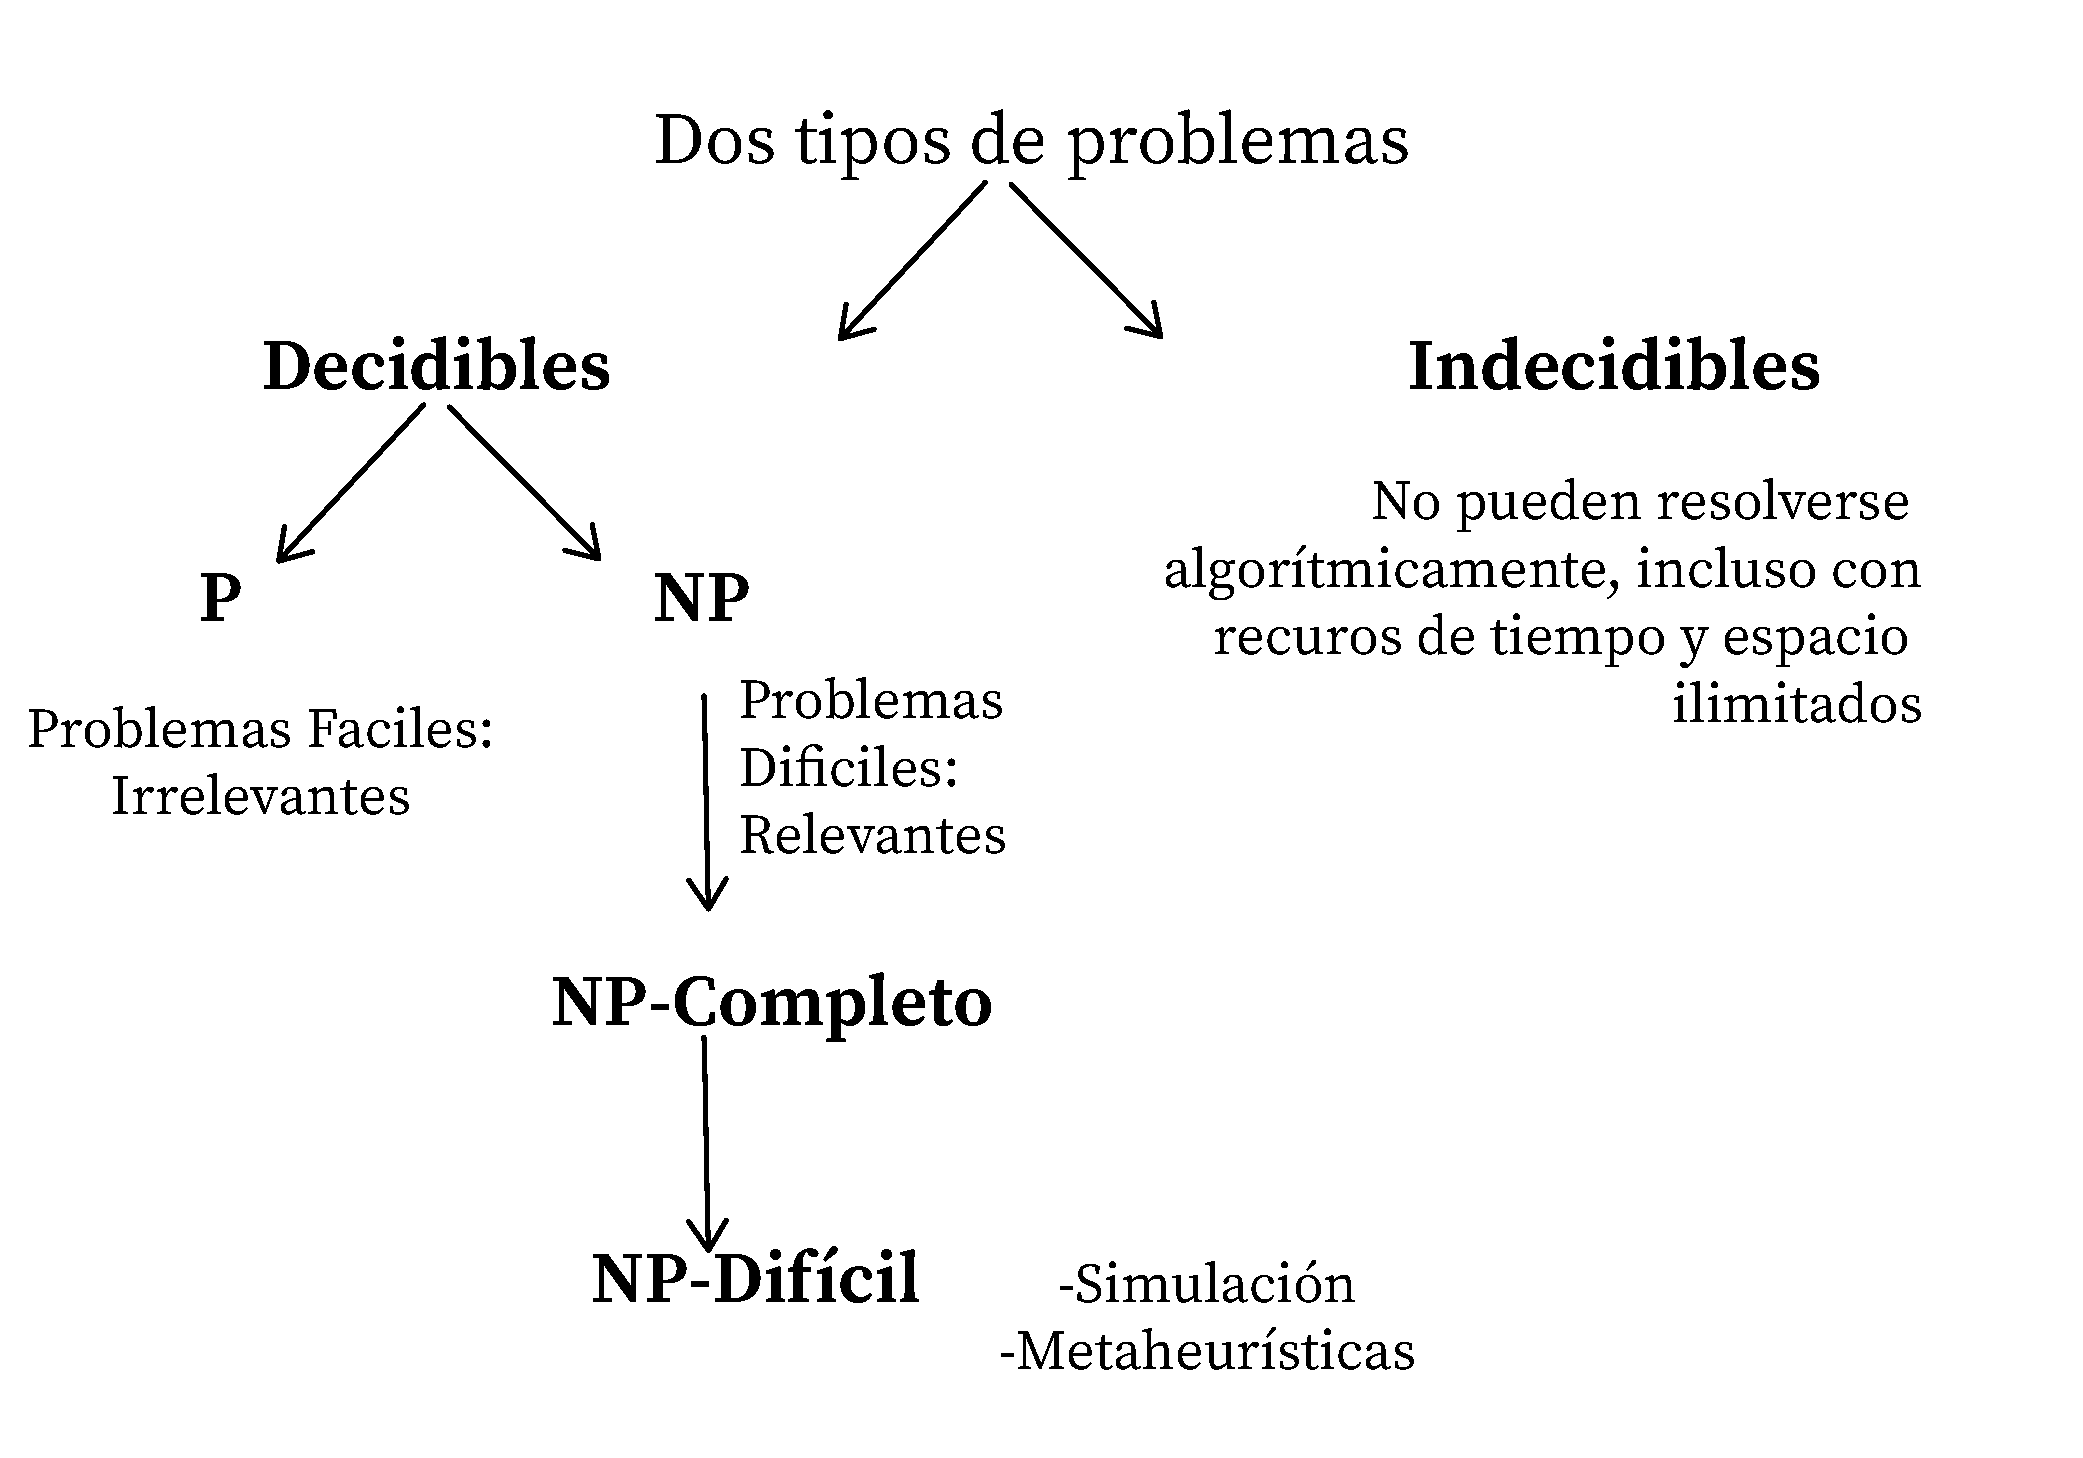
\includegraphics[width=0.6\textwidth]{Figuras/Diagrama.pdf}
	\caption{Clasificación de los problemas computacionales en decidibles e indecidibles~\citep{maldonado2013problema}.}
	\label{fig:decidibilidad}
\end{figure}

En este trabajo, los problemas abordados —el \textbf{TSP}, el \textbf{VRP} y el \textbf{VRP-TW}— son considerados \textbf{problemas decidibles}. A continuación, se presenta una clasificación más detallada dentro de esta categoría, basada en la teoría de la complejidad computacional.

% [Sigue tu sección de Clases P y NP...]

\subsubsection{Clases P y NP}

Dentro de los problemas decidibles, las clases \textbf{P} y \textbf{NP} juegan un papel fundamental \citep{maldonado2013problema}.

\subsubsection*{Clase P}
Un problema pertenece a la clase \emph{\textbf{P}} si puede resolverse mediante un algoritmo cuyo tiempo de ejecución está acotado por una función polinomial respecto al tamaño de la entrada. Formalmente, existe un polinomio \(p(n)\) y constantes \(\alpha, n_0 > 0\) tales que:

\[
	D(n) \leq \alpha \cdot p(n) \quad \forall n \geq n_0,
\]

lo que se expresa en notación asintótica como

\[
	D = O(n^k).
\]

Aunque se considera que algoritmos con tiempo polinomial son “\textit{eficientes}”, en la práctica el grado del polinomio importa, ya que un polinomio de grado muy alto puede ser inviable. Un ejemplo clásico de problema en \emph{\textbf{P}} es la multiplicación de números naturales \citep{Flores2014}.

\subsubsection*{Clase NP}
\label{subsec: clase_np}
Un problema pertenece a la clase \emph{\textbf{NP}} si, dado un candidato a solución (\textit{certificado}), es posible verificar su validez en tiempo polinomial. Es importante notar que esto no implica necesariamente que exista un algoritmo eficiente para encontrar la solución, sino que su validación es eficiente. Un ejemplo típico es el \textbf{TSP}: si se proporciona una ruta candidata, es fácil comprobar en tiempo polinomial la longitud total de la ruta para verificar si cumple cierta condición \citep{Flores2014}.

\subsubsection*{La gran incógnita: ¿P = NP?}
Una de las preguntas abiertas más importantes en ciencias de la computación es si \(\mathbf{P = NP}\) o \(\mathbf{P \neq NP}\), es decir, si todo problema cuya solución puede verificarse rápidamente también puede resolverse rápidamente. Esta cuestión tiene profundas implicaciones teóricas y prácticas \citep{maldonado2013problema}.

\subsubsection{NP-Completo y NP-Difícil}

Dentro de la clase \emph{\textbf{NP}} existe una subclase de problemas llamados \textbf{NP-completos}, que son los problemas más difíciles en \emph{\textbf{NP}}. Si se encontrara un algoritmo eficiente para cualquiera de ellos, entonces todos los problemas en \emph{NP} podrían resolverse eficientemente \citep{maldonado2013problema}.

Por otro lado, los problemas \textbf{NP-difíciles} pueden ser incluso más complejos que los \textbf{NP-completos}, ya que no requieren pertenecer a \emph{\textbf{NP}} (es decir, su solución no tiene por qué ser verificable en tiempo polinomial), pero son al menos tan difíciles como los problemas \textbf{NP-completos}. Pueden incluir problemas de decisión, búsqueda u optimización \citep{maldonado2013problema}.

\begin{figure}[H]
	\centering
	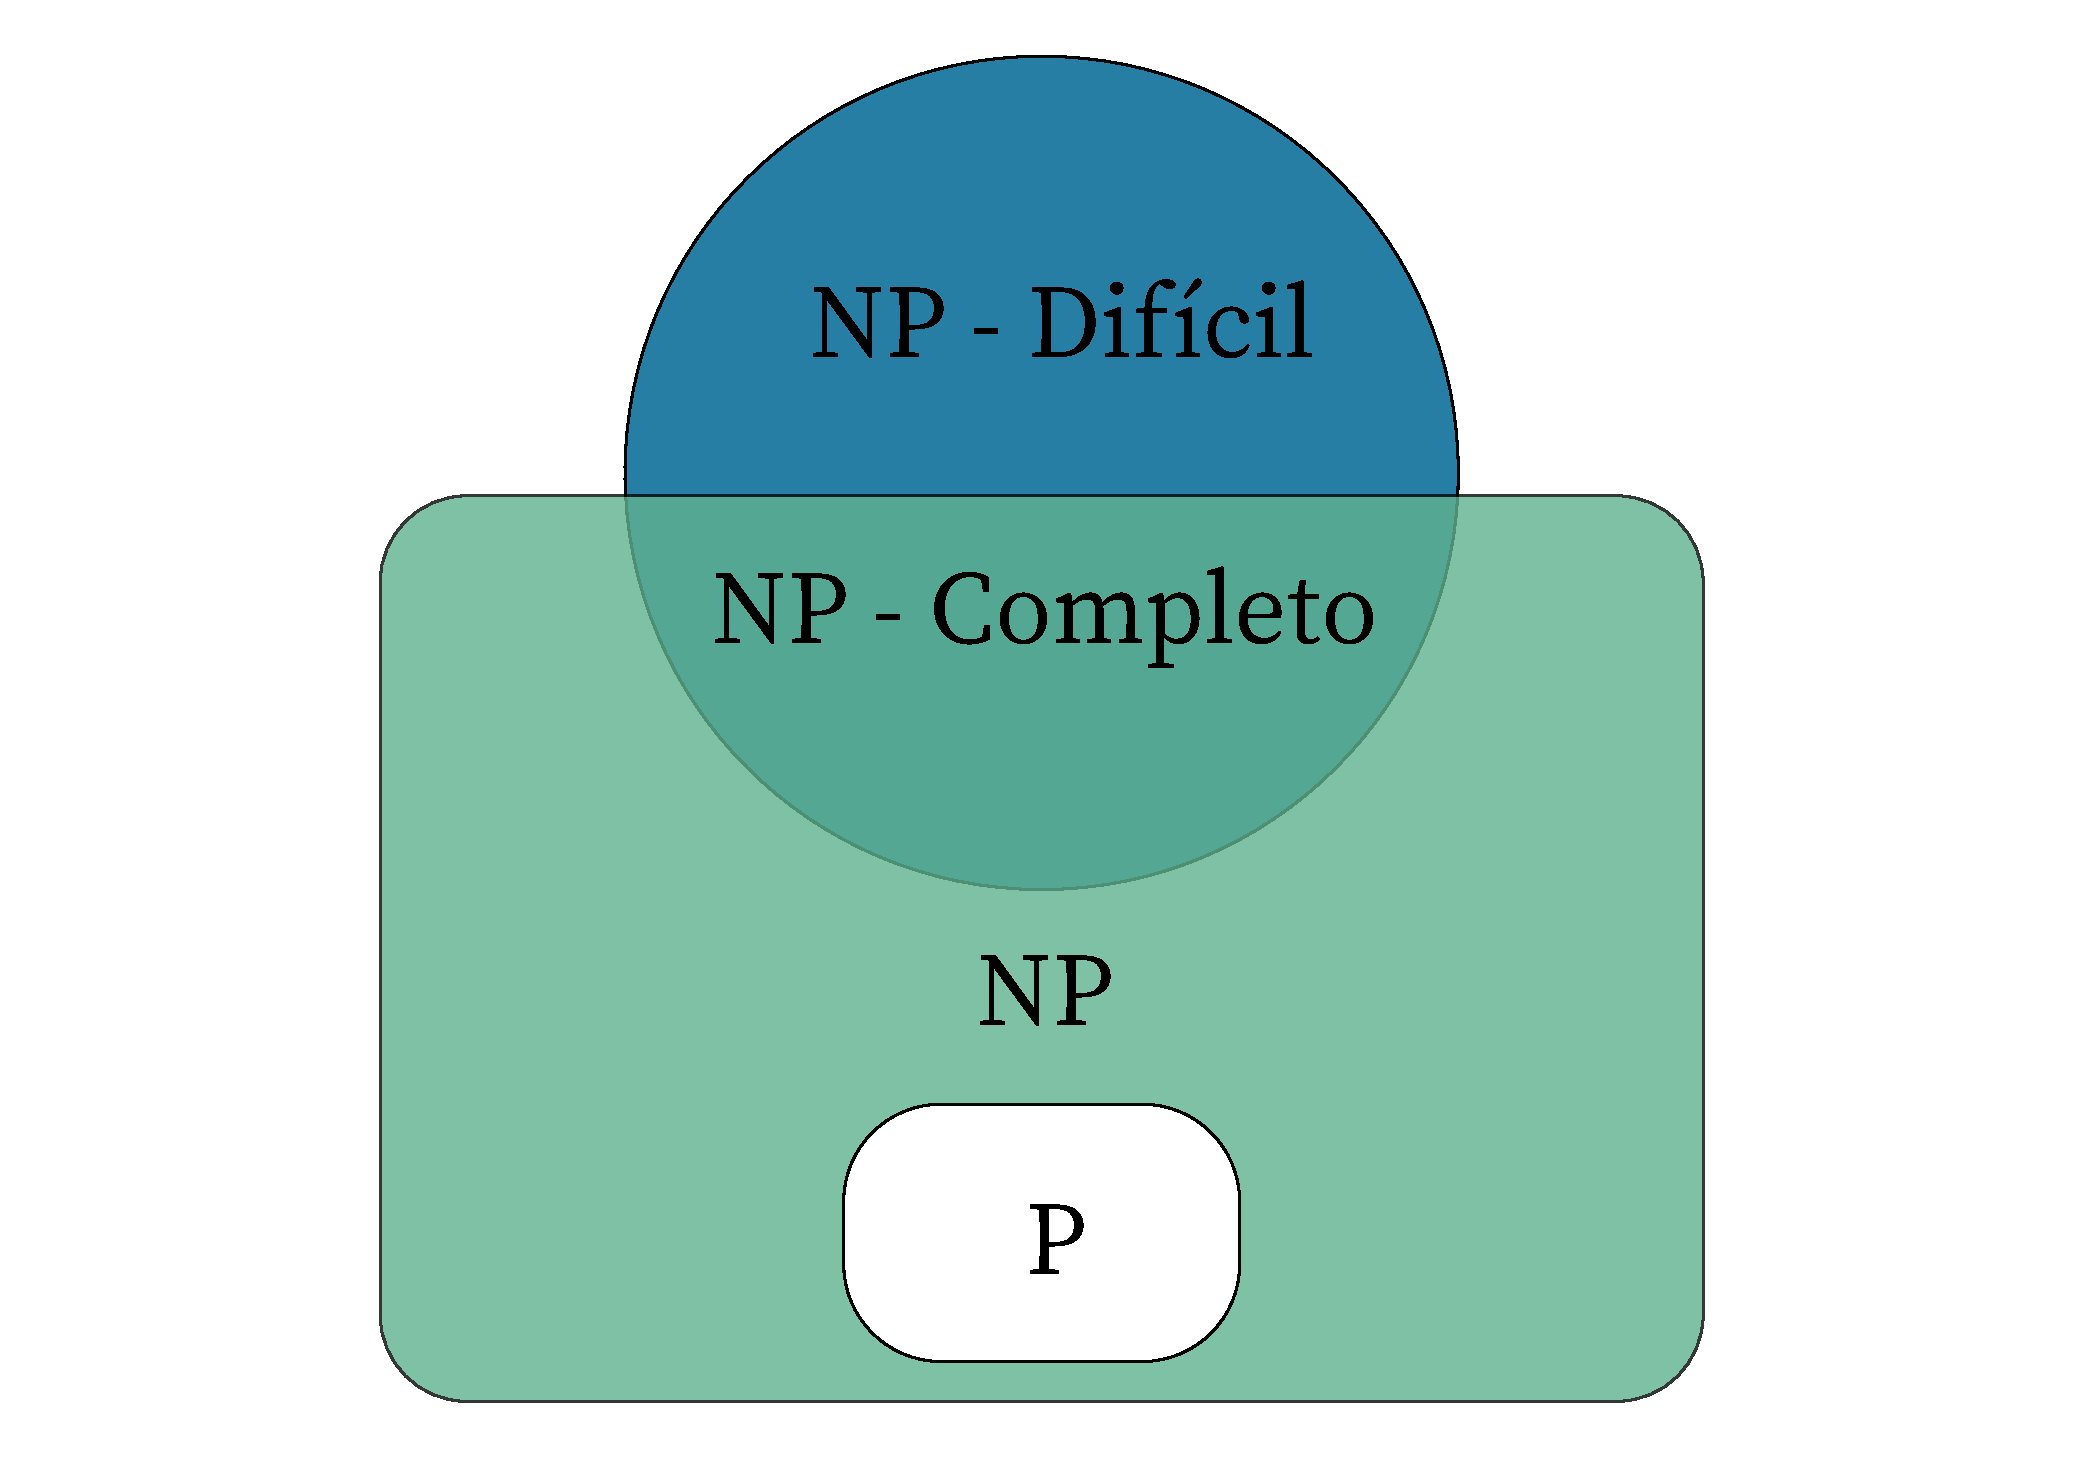
\includegraphics[width=0.6\textwidth]{Figuras/P_vs_NP.pdf}
	\caption{Relación entre las clases de complejidad: P, NP, NP-completo y NP-difícil.}
	\label{fig:p_vs_np}
\end{figure}

El crecimiento exponencial del tiempo requerido para resolver problemas como el \textbf{TSP}, el \textbf{VRP} y el \textbf{VRP-TW} los ubica dentro de la clase \emph{\textbf{NP}}. Estos problemas, aunque decidibles, presentan una complejidad tan elevada que no se conoce ningún algoritmo exacto que los resuelva eficientemente para instancias grandes. Por ello, más adelante se analizará su clasificación específica dentro de \emph{\textbf{NP}}, así como las estrategias metaheurísticas empleadas para aproximar soluciones en tiempos razonables.

\subsection{Problemas de Optimización Combinatoria}

De manera complementaria a la definición formal presentada en la sección~\ref{subsec:opt_discreta}, Papadimitriou y Steiglitz \citep{papadimitriou1998} definen la \textbf{optimización combinatoria} como el estudio de problemas de optimización en los que el conjunto de soluciones factibles es discreto, o puede discretizarse mediante un proceso de enumeración, y donde se busca una solución que optimice una función objetivo definida sobre dicho conjunto.

Los problemas de optimización combinatoria constituyen una clase amplia de modelos aplicables a diversas áreas, especialmente en la planificación y el enrutamiento de vehículos. Dentro de este campo destacan el \textbf{TSP}, que representa la forma más básica de optimización de rutas, y sus extensiones, que incorporan restricciones adicionales propias de escenarios reales, como la capacidad limitada de los vehículos o las ventanas de tiempo en las que deben realizarse las entregas.

En este contexto, el \textbf{VRP} y el \textbf{VRP-TW} se han consolidado como dos de los desafíos más estudiados, debido a su relevancia práctica y su elevada complejidad computacional. A continuación, se describen estos problemas en detalle.
\subsubsection{Problema del Agente Viajero (TSP)}
\label{subsec:problem_tsp}

El \textbf{Problema del Agente Viajero}, conocido por sus siglas en inglés como \textbf{\textit{TSP} (\emph{Travelling Salesman Problem})}, es uno de los problemas más reconocidos y complejos dentro de las ciencias computacionales. Ha sido estudiado desde diversas ramas de la ingeniería y por múltiples motivos. Su aplicación principal consiste en determinar rutas desde diferentes enfoques, ya sea en procesos que requieren una secuencia específica o en operaciones logísticas relacionadas con el transporte, con el objetivo de encontrar la ruta óptima considerando criterios de minimización de distancia o de costo \citep{lopez2014tabu}.

En la Figura~\ref{fig:tsp} se presenta una representación gráfica de una posible solución al \textbf{TSP}. En ella, un vehículo parte de un nodo inicial(depósito), recorre una serie de ciudades o puntos de entrega siguiendo una secuencia determinada, y regresa al punto de partida, completando así un circuito cerrado que minimiza la distancia total recorrida.

\begin{figure}[H]
	\centering
	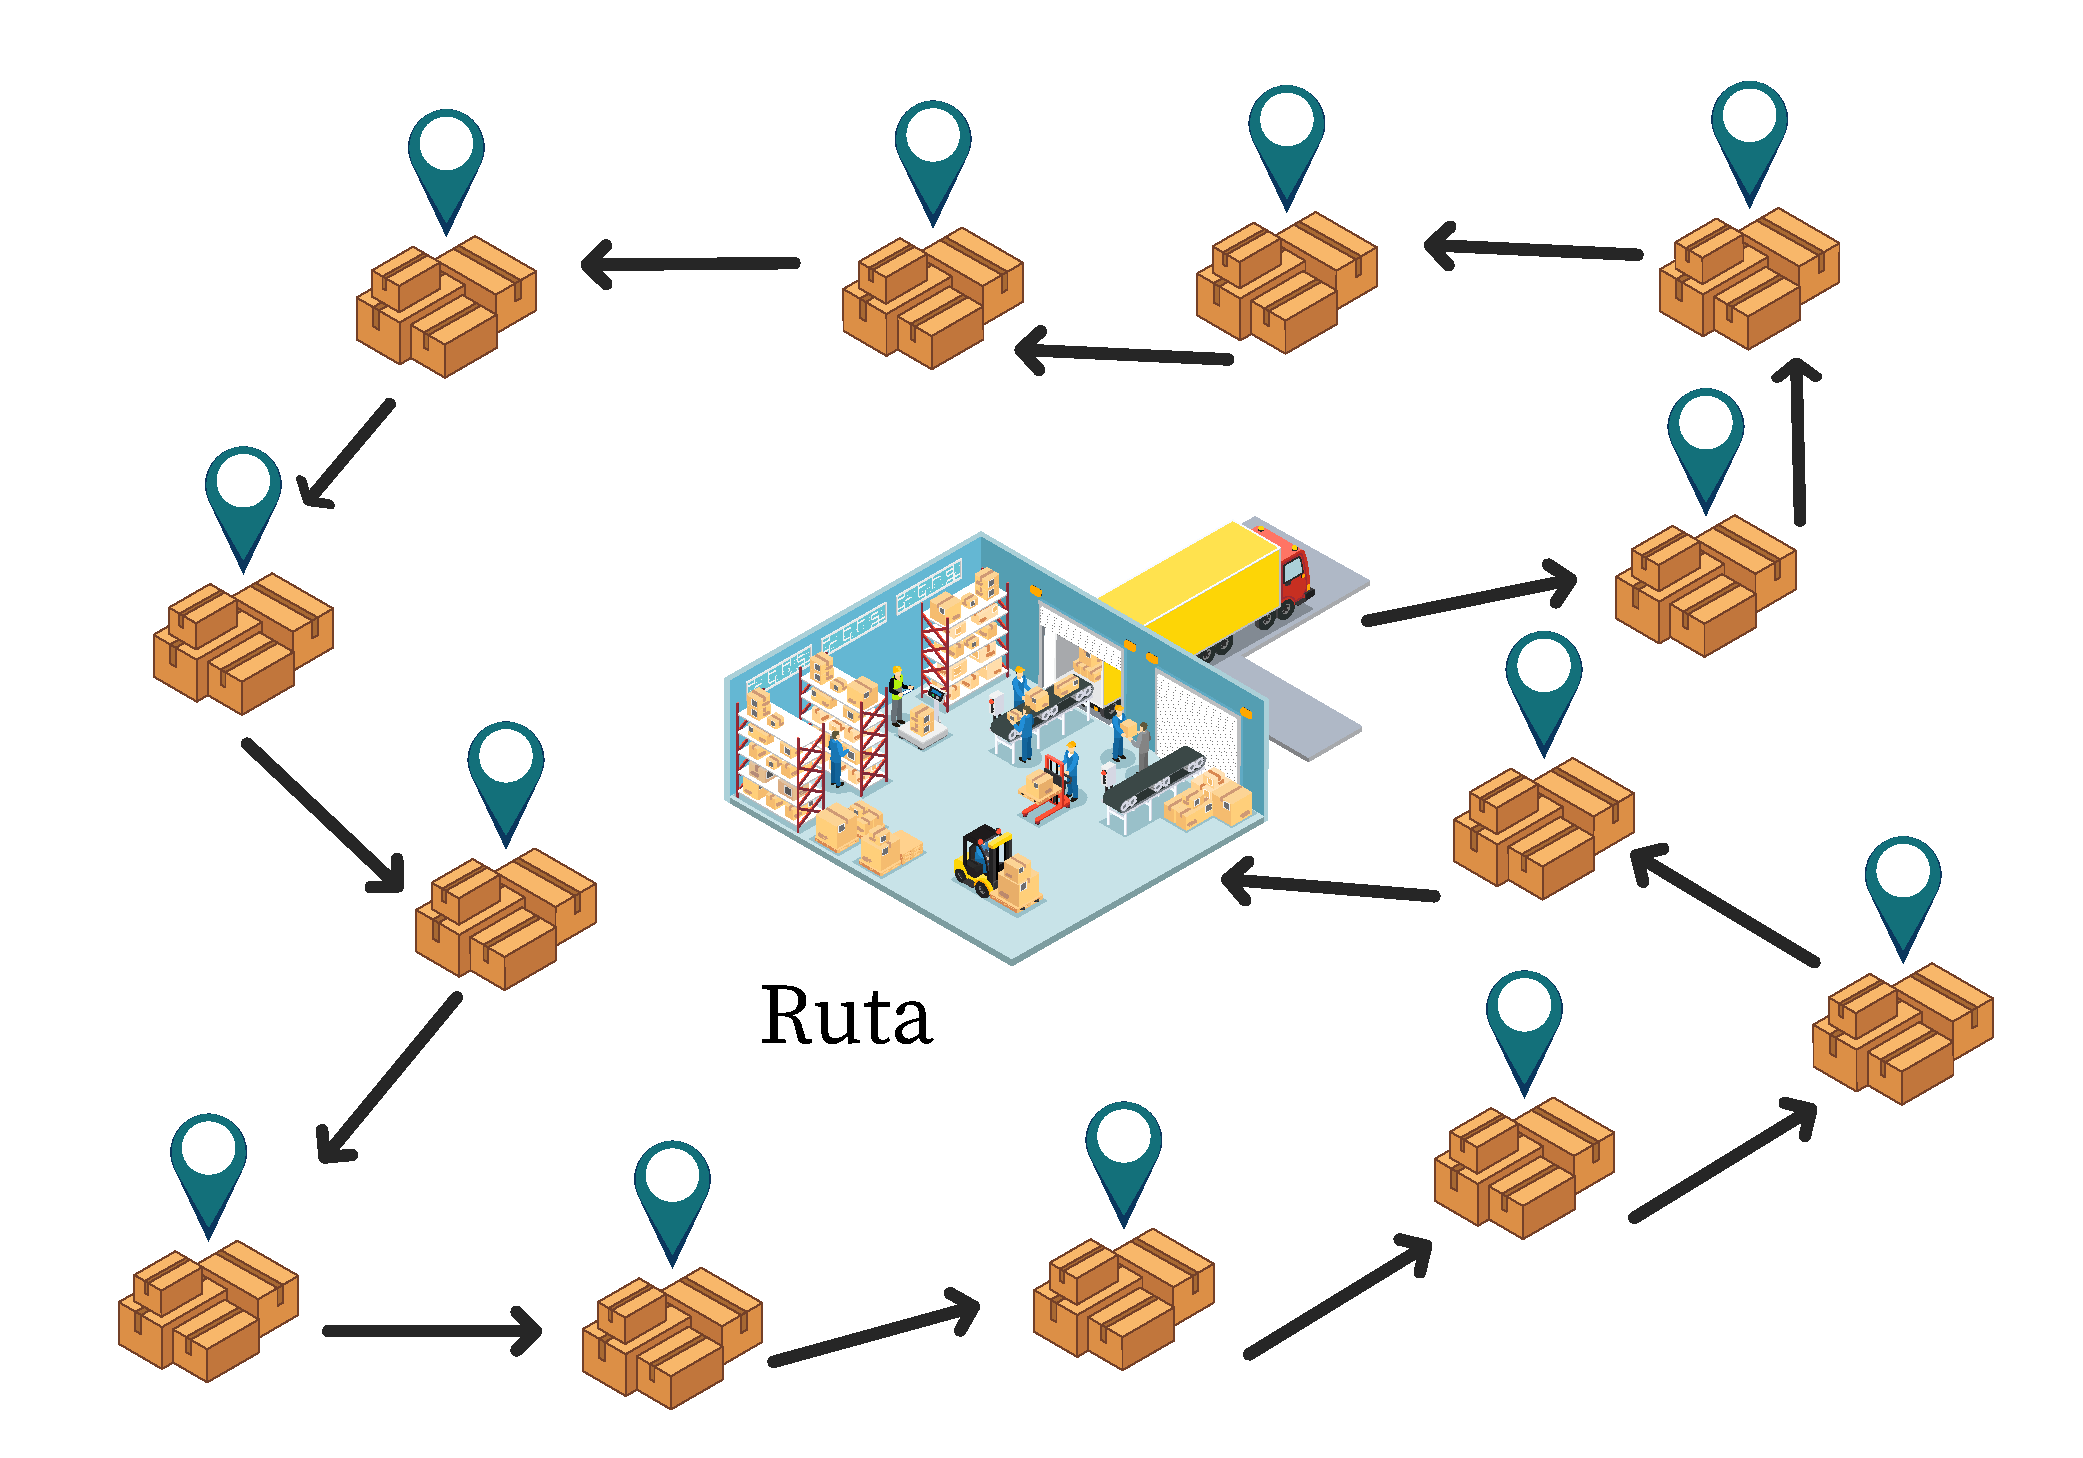
\includegraphics[width=0.6\textwidth]{Figuras/TSP.pdf}
	\caption{Ejemplificación de una solución al Problema del Agente Viajero (TSP).}
	\label{fig:tsp}
\end{figure}



Según \citep{torres2018}, el \textbf{TSP} se define sobre un grafo \(G = [N,A,C]\), donde \(N\) es el conjunto de nodos, \(A\) es el conjunto de arcos y \(C = [c_{ij}]\) es la matriz de costos (distancias) entre nodos \(i\) y \(j\). El objetivo es encontrar un ciclo hamiltoniano de costo mínimo que recorra todos los nodos una sola vez y regrese al punto de partida.

\subsubsection*{Modelo Matemático del Problema del Agente Viajero (TSP)}

\begin{equation}
	\min \sum_{i=1}^N \sum_{j=1}^N c_{ij}\,x_{ij}
	\label{eq:TSP_obj}
\end{equation}
\addcontentsline{eq}{myequations}{\protect\numberline{\theequation}Función objetivo TSP: minimizar el costo total del recorrido}

sujeto a:

\begin{equation}
	\sum_{j=1}^N x_{ij} = 1, \quad \forall i = 1,\dots,N
	\label{eq:TSP_out}
\end{equation}
\addcontentsline{eq}{myequations}{\protect\numberline{\theequation}Restricción de salida única de cada nodo}

\begin{equation}
	\sum_{i=1}^N x_{ij} = 1, \quad \forall j = 1,\dots,N
	\label{eq:TSP_in}
\end{equation}
\addcontentsline{eq}{myequations}{\protect\numberline{\theequation}Restricción de entrada única a cada nodo}

\begin{equation}
	u_i - u_j + N x_{ij} \leq N - 1, \quad \forall i,j = 2,\dots,N, \; i \neq j
	\label{eq:TSP_subtour}
\end{equation}
\addcontentsline{eq}{myequations}{\protect\numberline{\theequation}Restricción de eliminación de subciclos}

\begin{equation}
	x_{ij} \in \{0,1\}, \quad \forall i,j = 1,\dots,N
	\label{eq:TSP_bin}
\end{equation}
\addcontentsline{eq}{myequations}{\protect\numberline{\theequation}Variables binarias que indican si la ruta va de \(i\) a \(j\)}

\medskip

\noindent donde:
\begin{itemize}
	\item \(x_{ij} = 1\) si la ruta va de \(i\) a \(j\), y 0 en caso contrario;
	\item \(u_i\) son variables auxiliares usadas para eliminar subciclos, con \(i=2,\dots,N\) \citep{torres2018}.
\end{itemize}

La \textbf{función objetivo}~\eqref{eq:TSP_obj} representa la suma total de los costos (o distancias) de los arcos que conforman el recorrido. \textbf{La restricción} en~\eqref{eq:TSP_out} garantizan que, al salir de cada nodo, sólo se dirija a un único nodo siguiente. \textbf{La restricción} en~\eqref{eq:TSP_in} aseguran que a cada nodo únicamente se llegue una vez. \textbf{La restricción}~\eqref{eq:TSP_subtour} es fundamental, ya que previene la formación de subciclos que no incluyan a todos los nodos, asegurando así un recorrido único y completo.Finalmente, \textbf{la restricción}~\eqref{eq:TSP_bin} indica que las variables \(x_{ij}\) son binarias, es decir, sólo pueden tomar los valores 0 o 1, lo que permite representar la inclusión o exclusión de una ruta entre nodos \citep{torres2018}.

\subsubsection*{Complejidad del TSP}

Como explica \cite{papadimitriou1998}, el \textbf{TSP} es \textit{NP-difícil}, y su versión de decisión es \textit{NP-completa}. Esto implica que la búsqueda de un algoritmo eficiente para resolverlo representa un desafío fundamental en la teoría de la computación, pues encontrar una solución polinomial para el \textbf{TSP} permitiría resolver eficientemente toda la clase \textit{NP}. Esta dificultad justifica la utilización de algoritmos heurísticos y metaheurísticos, dado que las técnicas exactas sólo resultan prácticas para instancias

El \textbf{TSP} ha sido tradicionalmente considerado como el punto de partida para el estudio de problemas más complejos de enrutamiento, como el \textbf{VRP} y sus variantes, entre ellas el  \textbf{VRP-TW}. Su análisis proporciona una base conceptual sólida para comprender aspectos fundamentales como la construcción de rutas, la minimización de costos y el manejo de restricciones operativas. Estudiar el \textbf{TSP} permite introducir de forma gradual nuevas variables y condiciones, lo que lo convierte en un modelo introductorio ideal para el desarrollo de enfoques logísticos más realistas.

\subsubsection{Problema del Problema Ruteo de Vehículos (VRP)}
\label{subsec:problem_vrp}

El \textbf{Problema del Ruteo de Vehículos}, conocido por sus siglas en inglés como \textbf{\textit{VRP} (\emph{Vehicle Routing Problem})}, puede interpretarse como la convergencia de dos problemas clásicos de optimización combinatoria: el \textbf{Problema del Agente Viajero (TSP)} mencionado anteriormene en la sección~\ref{subsec:problem_tsp}, en el que se asume una capacidad infinita de los vehículos, y el \textbf{Problema de Empaquetamiento en Compartimentos (BPP)} \cite{daza2009}. En su formulación más básica, el \textbf{VRP} considera un depósito central desde donde parte una flota de vehículos para atender a un conjunto de clientes distribuidos geográficamente. Cada vehículo debe visitar un subconjunto de clientes exactamente una vez, respetando su capacidad de carga y satisfaciendo la demanda de los clientes asignados. El objetivo es minimizar el costo total asociado a las rutas, las cuales inician y finalizan en el depósito \cite{montes2017}.

La Figura~\ref{fig:vrp} muestra una representación gráfica de una solución al \textbf{VRP}. En este ejemplo, varios vehículos parten desde un depósito central para atender a distintos clientes distribuidos geográficamente. Cada ruta ha sido asignada de manera que se respeten las restricciones de capacidad de carga de los vehículos, y se minimice la distancia total recorrida, cumpliendo así con los objetivos del problema.

\begin{figure}[H]
	\centering
	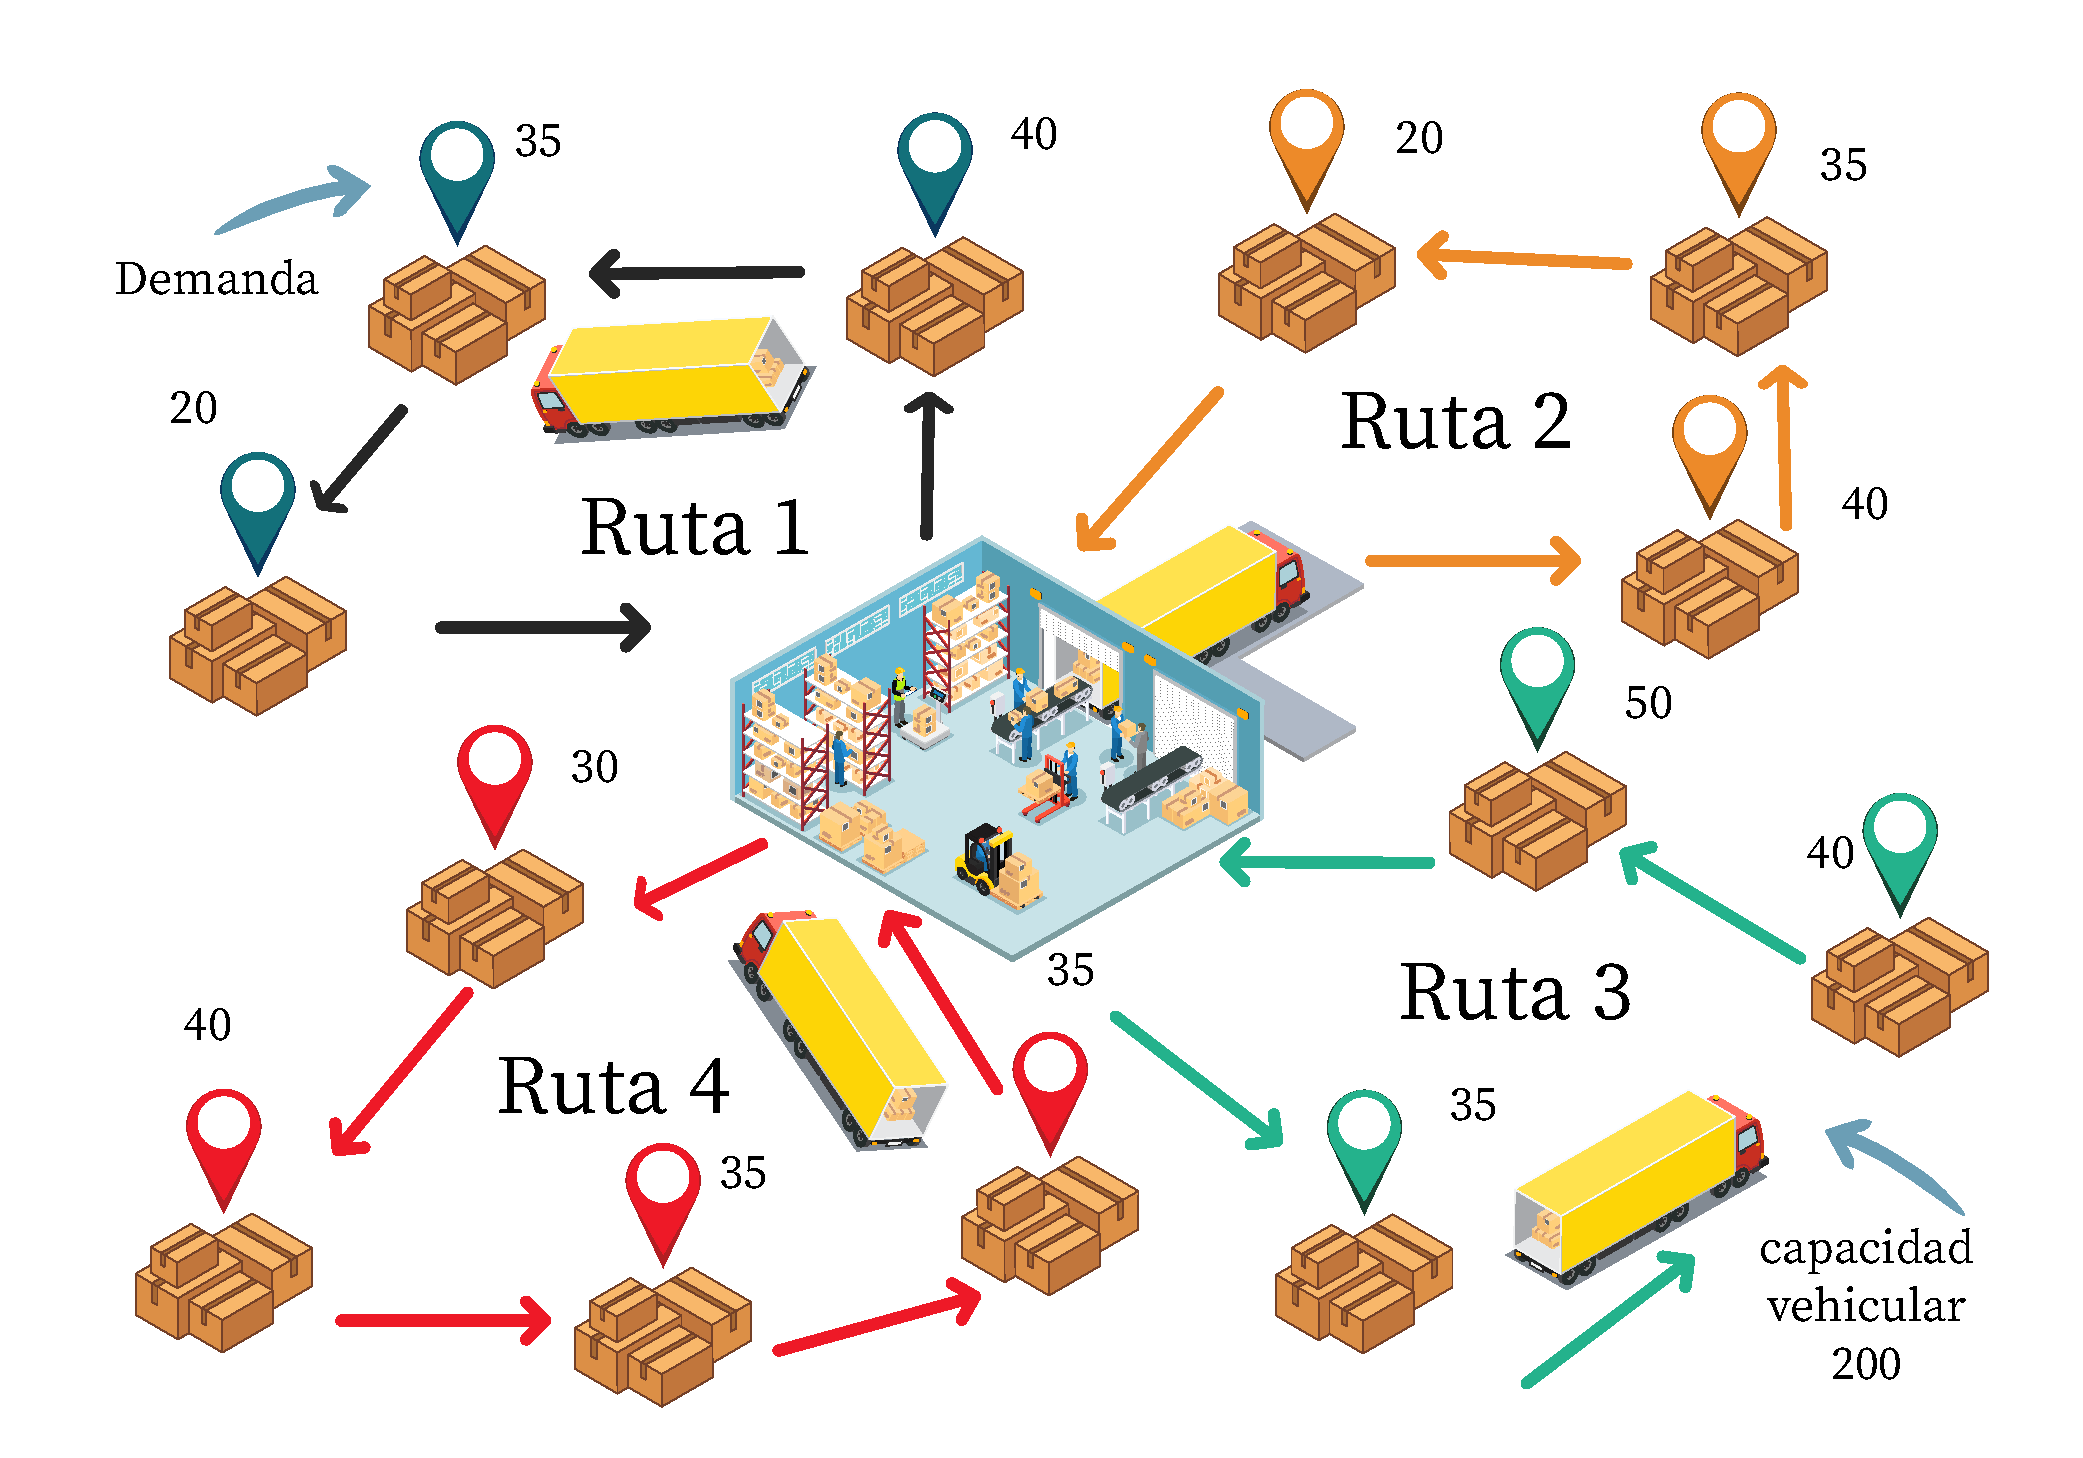
\includegraphics[width=0.6\textwidth]{Figuras/VRP.pdf}
	\caption{Ejemplificación de una solución al Problema de Ruteo de Vehículos (VRP).}
	\label{fig:vrp}
\end{figure}

Según \citep{toth2014}, el \textbf{VRP}  se define sobre un grafo $G = (V, A)$, donde $V = \{0, 1, \dots, n\}$ representa el conjunto de nodos, con el nodo $0$ correspondiente al depósito y los nodos restantes a los clientes, $A$ es el conjunto de arcos, y $C = [c_{ij}]$ es la matriz de costos asociados a los arcos $(i, j)$. El objetivo es determinar un conjunto de rutas de costo mínimo para una flota de vehículos idénticos, de modo que: cada cliente sea visitado exactamente una vez por un solo vehículo, cada ruta comience y termine en el depósito, y la demanda total de los clientes en cada ruta no exceda la capacidad del vehículo.

\subsubsection*{Modelo Matemático del Problema de Ruteo de Vehículos (VRP)}

\begin{equation}
	\min \sum_{i \in V} \sum_{j \in V} c_{ij} x_{ij}
	\label{eq:VRP_obj}
\end{equation}
\addcontentsline{eq}{myequations}{\protect\numberline{\theequation}Función objetivo VRP: minimizar el costo total del recorrido}

sujeto a:

\begin{equation}
	\sum_{i \in V} x_{ij} = 1, \quad \forall j \in V \setminus \{0\}
	\label{eq:VRP_in}
\end{equation}
\addcontentsline{eq}{myequations}{\protect\numberline{\theequation}Restricción: entrada única a cada cliente}

\begin{equation}
	\sum_{j \in V} x_{ij} = 1, \quad \forall i \in V \setminus \{0\}
	\label{eq:VRP_out}
\end{equation}
\addcontentsline{eq}{myequations}{\protect\numberline{\theequation}Restricción: salida única desde cada cliente}

\begin{equation}
	\sum_{i \in V} x_{i0} = K
	\label{eq:VRP_into_depot}
\end{equation}
\addcontentsline{eq}{myequations}{\protect\numberline{\theequation}Restricción: número de vehículos que regresan al depósito}

\begin{equation}
	\sum_{j \in V} x_{0j} = K
	\label{eq:VRP_from_depot}
\end{equation}
\addcontentsline{eq}{myequations}{\protect\numberline{\theequation} Restricción: número de vehículos que salen del depósito}

\begin{equation}
	\sum_{i \in S} \sum_{j \in S} x_{ij} \geq r(S), \quad \forall S \subseteq V \setminus \{0\},\; S \neq \emptyset
	\label{eq:VRP_subtour}
\end{equation}
\addcontentsline{eq}{myequations}{\protect\numberline{\theequation} Restricción de conectividad: eliminación de subrutas}

\begin{equation}
	x_{ij} \in \{0, 1\}, \quad \forall i,j \in V
	\label{eq:VRP_bin}
\end{equation}
\addcontentsline{eq}{myequations}{\protect\numberline{\theequation} Variables binarias: decisión de ruta entre nodos}
\medskip

\noindent donde:
\begin{itemize}
	\item \(V\) es el conjunto de nodos (clientes más depósito), con el depósito representado por el nodo 0;
	\item \(c_{ij}\) es el costo (o distancia) de viajar del nodo \(i\) al nodo \(j\);
	\item \(x_{ij} = 1\) si se viaja directamente del nodo \(i\) al nodo \(j\), 0 en otro caso;
	\item \(K\) es el número de vehículos disponibles en el depósito;
	\item \(S\) es un subconjunto de clientes, y \(r(S)\) representa el número mínimo de vehículos necesarios para satisfacer la demanda total de los clientes en \(S\) \citep{toth2014}.
\end{itemize}

La \textbf{función objetivo}~\eqref{eq:VRP_obj} minimiza el costo total de todas las rutas. \textbf{Las restricciones}~\eqref{eq:VRP_in} y~\eqref{eq:VRP_out} aseguran que cada cliente sea visitado exactamente una vez. \textbf{Las restricciones}~\eqref{eq:VRP_into_depot} y~\eqref{eq:VRP_from_depot} controlan el número de vehículos que entran y salen del depósito. \textbf{La restricción}~\eqref{eq:VRP_subtour} evita la formación de subrutas que no incluyan al depósito, garantizando conectividad. Finalmente, \textbf{la restricción}~\eqref{eq:VRP_bin} indica que las variables de decisión son binarias \citep{toth2014}.


\subsubsection*{Complejidad del VRP}
\label{subsec:complejidad_vrp}

Como señalan Laporte y Nobert \cite{laporte1987}, el \textbf{VRP} es \textit{NP-difícil}, incluso en su versión más simple con un solo vehículo (es decir, el \textbf{TSP}). Esto significa que no se conoce ningún algoritmo que lo resuelva de forma exacta en tiempo polinomial, y su complejidad crece exponencialmente con el número de clientes. Por ello, la mayoría de las instancias prácticas requieren el uso de técnicas heurísticas o metaheurísticas, ya que los métodos exactos son computacionalmente inviables para problemas de tamaño medio o grande.

El \textbf{VRP} representa la extensión natural del \textbf{TSP} hacia escenarios logísticos más realistas y complejos, incorporando restricciones operativas que reflejan las limitaciones del mundo real. Su estudio es fundamental para comprender cómo las restricciones de capacidad, múltiples vehículos y la gestión de flotas impactan en la optimización de rutas. El \textbf{VRP} sirve como base conceptual para abordar problemas logísticos avanzados como la distribución con ventanas de tiempo, el ruteo con múltiples depósitos y la optimización de última milla en el comercio electrónico. Analizar el \textbf{VRP} permite desarrollar una comprensión profunda de los trade-offs entre minimización de costos, utilización eficiente de recursos y satisfacción de restricciones operativas, estableciendo los fundamentos teóricos necesarios para abordar las complejidades de los sistemas de distribución modernos.

\subsubsection{Problema de Ruteo de Vehículos con Ventanas de Tiempo (VRP-TW)}
\label{subsec:problem_vrptw}

El \textbf{Problema de Ruteo de Vehículos con Ventanas de Tiempo}, conocido por sus siglas en inglés como \textbf{VRP-TW (\textit{Vehicle Routing Problem with Time Windows})}, es una extensión del clásico \textbf{VRP} mencionado anteriormene en la sección~\ref{subsec:problem_vrp} que incorpora restricciones temporales. En este problema, además de satisfacer las demandas específicas de cada cliente, es imprescindible que las visitas se realicen dentro de una franja horaria determinada para cada uno de ellos \citep{toth2014}. Específicamente, el servicio a un cliente debe comenzar en un instante mayor o igual al inicio de su ventana de tiempo, y el arribo al punto de servicio no puede exceder el límite superior de dicha ventana. Asimismo, en caso de que un vehículo llegue antes del inicio de la ventana, deberá esperar hasta el momento indicado para poder atender al cliente \citep{montes2017}.

En este contexto, el objetivo fundamental del \textbf{VRP-TW} es determinar un conjunto de rutas para una flota de vehículos homogéneos que partan y regresen al depósito, visiten cada cliente exactamente una vez dentro de su respectiva ventana temporal, y sin exceder la capacidad de los vehículos. Todo esto debe lograrse minimizando el costo total del recorrido, usualmente expresado en términos de distancia o tiempo \cite{solomon1987algorithms}.

En la Figura~\ref{fig:vrptw} se muestra una solución típica al \textbf{VRP-TW}. En este caso, las rutas de múltiples vehículos parten desde un único depósito, deben cumplir con las capacidades máximas y además respetar las ventanas temporales de atención en cada cliente, optimizando el recorrido total.

\begin{figure}[H]
	\centering
	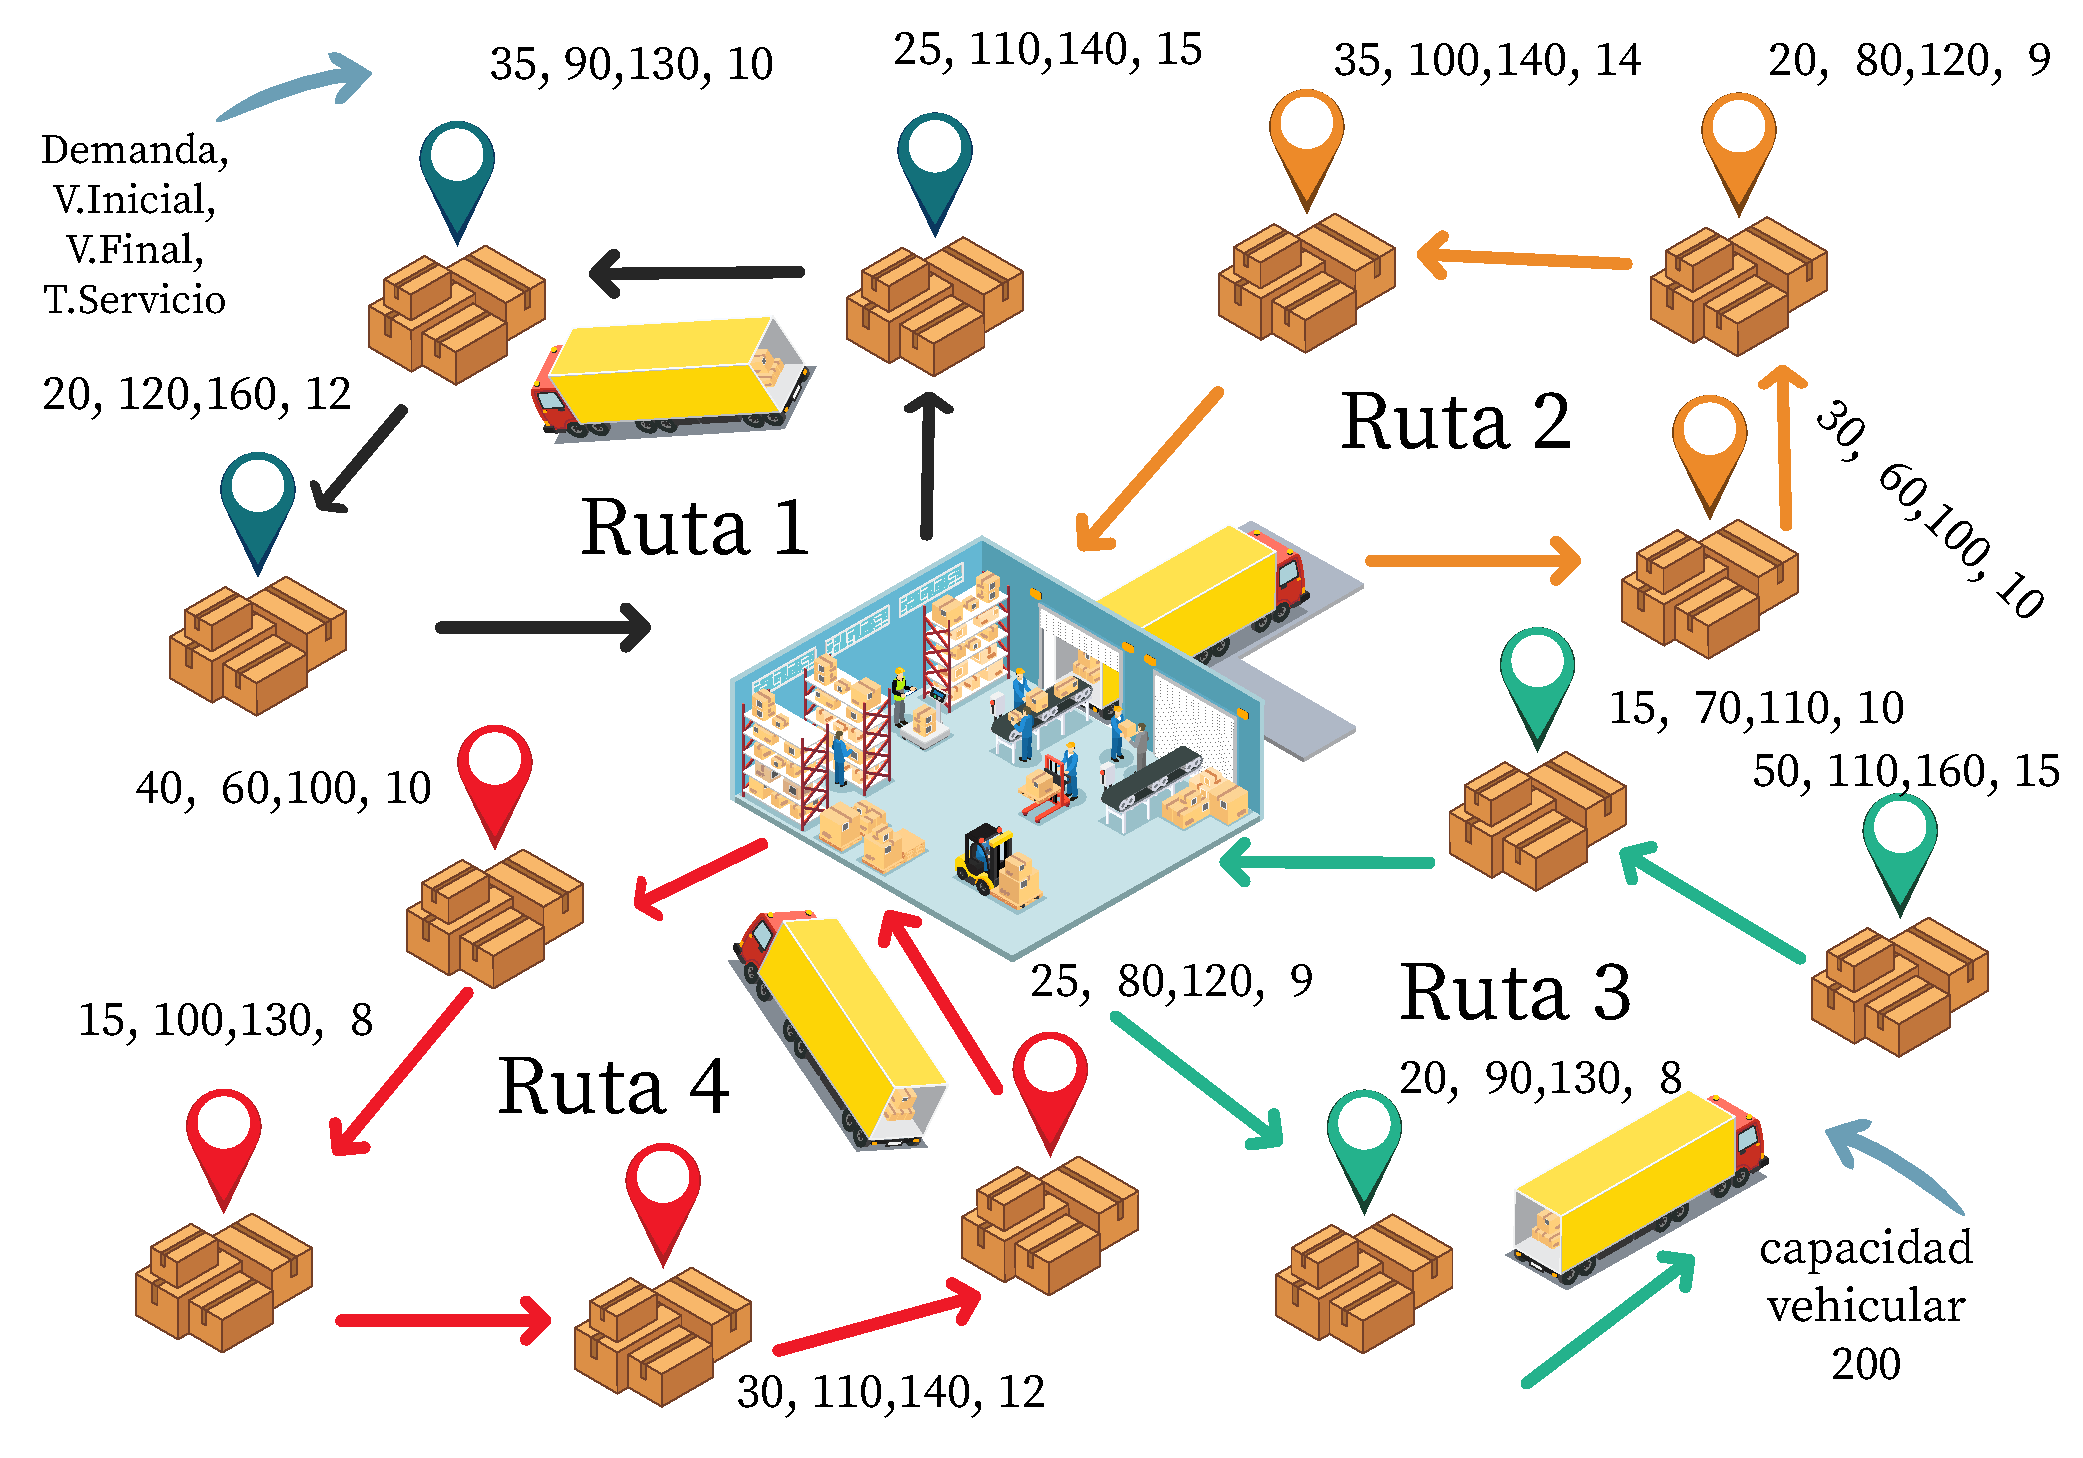
\includegraphics[width=0.6\textwidth]{Figuras/VRPTW.pdf}
	\caption{Ejemplificación de una solución al Problema de Ruteo de Vehículos con Ventanas de Tiempo (VRP-TW).}
	\label{fig:vrptw}
\end{figure}

Según \citep{toth2014}, el \textbf{VRP-TW} se define sobre un grafo dirigido \(G = (V, A)\), donde \(V = \{0, 1, \dots, n, n+1\}\) representa el conjunto de nodos, siendo \(0\) y \(n+1\) el depósito (nodos origen y destino, respectivamente), y \(N = V \setminus \{0, n+1\}\) el conjunto de clientes. Cada arco \((i, j) \in A\) tiene asociado un costo \(c_{ij}\) y un tiempo de viaje \(t_{ij}\). Además, cada cliente \(i\) tiene una demanda \(d_i\), un tiempo de servicio \(s_i\), y una ventana de tiempo \([a_i, b_i]\) dentro de la cual debe iniciarse su servicio.


\subsubsection*{Modelo Matemático del Problema de Ruteo de Vehículos con Ventanas de Tiempo(VRP-TW)}

\begin{equation}
	\min \sum_{k \in K} \sum_{i \in V} \sum_{j \in V} c_{ij} x_{ijk}
	\label{eq:VRPTW_obj}
\end{equation}
\addcontentsline{eq}{myequations}{\protect\numberline{\theequation} Función objetivo VRPTW: minimizar el costo total del recorrido}

sujeto a:

\begin{equation}
	\sum_{k \in K} \sum_{j \in V} x_{ijk} = 1, \quad \forall i \in N
	\label{eq:VRPTW_visit_once}
\end{equation}
\addcontentsline{eq}{myequations}{\protect\numberline{\theequation} Restricción: cada cliente es visitado exactamente una vez}

\begin{equation}
	\sum_{j \in V} x_{0jk} = 1, \quad \forall k \in K
	\label{eq:VRPTW_start_depot}
\end{equation}
\addcontentsline{eq}{myequations}{\protect\numberline{\theequation} Restricción: cada vehículo inicia su ruta en el depósito}

\begin{equation}
	\sum_{i \in V} x_{i,n+1,k} = 1, \quad \forall k \in K
	\label{eq:VRPTW_end_depot}
\end{equation}
\addcontentsline{eq}{myequations}{\protect\numberline{\theequation} Restricción: cada vehículo termina su ruta en el depósito}

\begin{equation}
	\sum_{j \in V} x_{ijk} - \sum_{j \in V} x_{jik} = 0, \quad \forall k \in K, \forall i \in N
	\label{eq:VRPTW_flow_balance}
\end{equation}
\addcontentsline{eq}{myequations}{\protect\numberline{\theequation} Restricción: conservación de flujo para cada vehículo y cliente}

\begin{equation}
	w_{jk} \geq w_{ik} + s_i + t_{ij} - M (1 - x_{ijk}), \quad \forall k \in K, \forall i,j \in V
	\label{eq:VRPTW_time_window}
\end{equation}
\addcontentsline{eq}{myequations}{\protect\numberline{\theequation} Restricción: respeto a la ventana de tiempo y orden de servicio}

\begin{equation}
	a_i \leq w_{ik} \leq b_i, \quad \forall k \in K, \forall i \in V
	\label{eq:VRPTW_time_bounds}
\end{equation}
\addcontentsline{eq}{myequations}{\protect\numberline{\theequation} Restricción: inicio del servicio dentro de la ventana de tiempo}

\begin{equation}
	\sum_{i \in V} \sum_{j \in V} d_i x_{ijk} \leq C, \quad \forall k \in K
	\label{eq:VRPTW_capacity}
\end{equation}
\addcontentsline{eq}{myequations}{\protect\numberline{\theequation} Restricción: capacidad máxima del vehículo}

\begin{equation}
	x_{ijk} \in \{0, 1\}, \quad w_{ik} \geq 0, \quad \forall k \in K, \forall i,j \in V
	\label{eq:VRPTW_bin}
\end{equation}
\addcontentsline{eq}{myequations}{\protect\numberline{\theequation} Variables binarias y tiempos no negativos}

\medskip
\noindent donde:
\begin{itemize}
	\item \(V = \{0, 1, \ldots, n, n+1\}\) es el conjunto de nodos, donde \(0\) y \(n+1\) representan el depósito;
	\item \(N = V \setminus \{0, n+1\}\) es el conjunto de clientes;
	\item \(K\) es el conjunto de vehículos disponibles;
	\item \(A\) es el conjunto de arcos permitidos entre nodos;
	\item \(c_{ij}\) es el costo o distancia de viajar del nodo \(i\) al nodo \(j\);
	\item \(x_{ijk}\) es variable binaria que indica si el vehículo \(k\) viaja directamente del nodo \(i\) al nodo \(j\);
	\item \(w_{ik}\) es el tiempo de inicio del servicio del vehículo \(k\) en el nodo \(i\);
	\item \(s_i\) es el tiempo de servicio requerido en el nodo \(i\);
	\item \(t_{ij}\) es el tiempo de viaje entre los nodos \(i\) y \(j\);
	\item \([a_i, b_i]\) es la ventana de tiempo para el nodo \(i\);
	\item \(d_i\) es la demanda del cliente \(i\);
	\item \(C\) es la capacidad máxima de cada vehículo;
	\item \(M\) es un número grande usado para activar o desactivar restricciones condicionales.
\end{itemize}

La \textbf{función objetivo}~\eqref{eq:VRPTW_obj} minimiza el costo total de todas las rutas. \textbf{Las restricciones}~\eqref{eq:VRPTW_visit_once} garantizan que cada cliente sea visitado exactamente una vez. \textbf{Las restricciones}~\eqref{eq:VRPTW_start_depot} y \eqref{eq:VRPTW_end_depot} aseguran que cada vehículo comience y termine su ruta en el depósito. \textbf{La restricción}~\eqref{eq:VRPTW_flow_balance} mantiene el balance de flujo para cada vehículo y cliente. \textbf{La restricción}~\eqref{eq:VRPTW_time_window} impone el orden y respeto a las ventanas temporales mediante los tiempos de servicio y de viaje, con ayuda del parámetro \(M\). \textbf{La restricción}~\eqref{eq:VRPTW_time_bounds} asegura que el servicio inicie dentro de la ventana asignada. \textbf{La restricción}~\eqref{eq:VRPTW_capacity} limita la capacidad máxima que puede transportar cada vehículo. Finalmente, \textbf{la restricción}~\eqref{eq:VRPTW_bin} define los dominios de las variables de decisión \citep{toth2014}.

\subsubsection*{Complejidad del VRP-TW}

Sabemos que la complejidad del \textbf{VRP} es \textit{NP-difícil}, como se señala en la \autoref{subsec:problem_vrp} y en \citep{laporte1987}. El \textbf{VRP-TW} es una generalización del \textbf{VRP} clásico, y también pertenece a la clase de problemas \textit{NP-difícil}. De hecho, incluso si se ignoran las ventanas de tiempo, el problema sigue siendo difícil de resolver. Al incorporar restricciones temporales, el \textbf{VRP-TW} se vuelve aún más complejo, tanto desde el punto de vista computacional como algorítmico. Según Bräysy y Gendreau \citep{braysy2005} y Toth y Vigo \citep{toth2014}, las ventanas de tiempo reducen significativamente el conjunto de soluciones viables, aumentando así la dificultad del problema.


El \textbf{VRP-TW} representa una evolución del \textbf{VRP} orientada a entornos donde las restricciones temporales son determinantes para la calidad del servicio. Esta variante refleja de forma más precisa los desafíos logísticos actuales, donde los clientes no solo deben ser visitados, sino también atendidos dentro de intervalos de tiempo específicos, lo cual impone una coordinación precisa entre la planificación de rutas, la gestión de recursos y el cumplimiento de niveles de servicio.

\subsection{Métodos de Solución para el VRP-TW}
Los problemas de enrutamiento como el \textbf{TSP}, el \textbf{VRP} y su extensión con ventanas de tiempo, el \textbf{VRP-TW}, mencionados en secciones anteriores, pertenecen a la clase de problemas \textit{NP-difíciles} \citep{papadimitriou1998, laporte1987, toth2014}. Esta clasificación se debe al crecimiento exponencial del tiempo requerido para resolverlos a medida que aumenta el número de nodos o clientes en la instancia.

Dada su complejidad computacional, estos problemas han sido abordados mediante diversas estrategias de solución que tienen como objetivo minimizar el costo total del recorrido, respetando las restricciones impuestas. Entre ellos se incluyen los \textit{métodos exactos}, así como las \textit{técnicas heurísticas y metaheurísticas}.

A continuación, se describen estos enfoques, junto con ejemplos representativos aplicados en los problemas mencionados.

\subsubsection{Métodos Exactos}

Son aquellos que parten de una formulación matemática del problema, generalmente como modelos de programación lineal entera o similares, y alcanzan soluciones factibles mediante algoritmos que acotan el conjunto de soluciones posibles \citep{luer2009}. Estos métodos garantizan la obtención de una solución óptima; sin embargo, su principal limitación radica en el alto costo computacional que implican, por lo que su eficiencia se restringe a instancias de tamaño reducido, de hasta aproximadamente 50 clientes en problemas de enrutamiento\citep{montes2017}.

Con base en la clasificación presentada por \citep{montes2017}, los métodos exactos pueden agruparse en las siguientes categorías:

\begin{enumerate}
	\item \textbf{Técnicas de relajación:} consisten en simplificar el modelo relajando ciertas restricciones complejas, lo que permite obtener cotas inferiores o superiores que guían la búsqueda de soluciones.
	\item \textbf{Búsqueda directa en árbol:} algoritmos como \emph{Branch and Bound} y \emph{Branch and Cut} exploran el espacio de soluciones mediante estructuras jerárquicas, descartando ramas no prometedoras.
	\item \textbf{Programación dinámica:} resuelve el problema descomponiéndolo en subproblemas más pequeños que se abordan de forma recursiva y eficiente.
	\item \textbf{Programación lineal entera:} utiliza modelos enteros mixtos como formulación clásica para problemas como el \textbf{VRP-TW}, y sirve frecuentemente de base para otros enfoques híbridos.
\end{enumerate}

Dado que el presente trabajo se enfoca en técnicas \textbf{\emph{heurísticas}} y \textbf{\emph{metaheurísticas}}, no se abordará en detalle la implementación de estos métodos exactos. Para una revisión más amplia, se remite al lector a \citep{montes2017}.

\subsubsection{Heurísticas}
\label{subsec:heuristica}

Heurística es un concepto cuyo origen se remonta a la Grecia clásica, derivado de la palabra griega \textit{heuriskein}, que significa encontrar o descubrir. Según la historia, se asocia con \textit{eureka}, la famosa exclamación atribuida a Arquímedes \citep{antonioSuarez2014}.

Para ejemplificar este concepto, se expone la siguiente definición:

\begin{quote}
	Según Zanakis et al.\ (citado en \citep{duarte2007metaheuristicas}), las heurísticas son \textit{``procedimientos simples, a menudo basados en el sentido común, que se supone que obtendrán una buena solución (no necesariamente óptima) a problemas difíciles de un modo sencillo y rápido''}.
\end{quote}

El desarrollo de las técnicas heurísticas clásicas aplicadas al \textbf{VRP-TW} se llevó a cabo principalmente entre las décadas de 1960 y 1990. Estas pueden clasificarse en tres categorías generales: \textit{métodos constructivos}, \textit{métodos de dos fases} y \textit{heurísticas de mejora} \citep{montes2017}, las cuales se describen a continuación.

\textbf{Métodos constructivos:} 
Las heurísticas constructivas elaboran progresivamente una solución factible, considerando los costos asociados en cada paso del proceso. Sin embargo, este tipo de métodos no incorpora una fase de mejora posterior sobre la solución obtenida \citep{toth2014}.

\textbf{Métodos de dos fases:} 
Las heurísticas de dos fases dividen el problema en dos componentes principales: la agrupación de vértices en rutas factibles y la construcción de dichas rutas, pudiendo existir retroalimentación entre ambas etapas. Estas técnicas se clasifican en dos enfoques: \textit{agrupación primero, ruta después} y \textit{ruta primero, agrupación después}. En el primer enfoque, los vértices se organizan inicialmente en grupos factibles y luego se construye una ruta vehicular para cada uno. En el segundo, se genera primero un recorrido global que abarca todos los vértices y posteriormente se segmenta en rutas factibles \citep{toth2014}.

En el presente trabajo se emplearon heurísticas basadas en los \textbf{métodos de mejora}, por lo que no se profundizará en los demás enfoques. Para una descripción más detallada, se recomienda consultar \citep{montes2017, toth2014, olivera2004heur}.

\textbf{Métodos de mejora:} 
Los métodos de mejora tienen como propósito optimizar una solución factible existente mediante una serie de intercambios o modificaciones de aristas y vértices, tanto dentro como entre rutas vehiculares, con el fin de disminuir el costo total del recorrido \citep{toth2014}.

Entre los operadores clásicos utilizados en los métodos de mejora para problemas de enrutamiento destacan los siguientes:

\begin{enumerate}
    \item \textbf{Operador de intercambio $\lambda$:} Consiste en eliminar $\lambda$ aristas de la solución y reconectar los $\lambda$ segmentos restantes. Una solución es óptima si no puede ser mejorada utilizando $\lambda$ intercambios \citep{olivera2004heur}.

    \item \textbf{Algoritmo de Lin-Kernighan:} Utiliza la idea de intercambiar un subconjunto de arcos por otro, donde dichos subconjuntos (y su cardinalidad) se modifican durante la ejecución del algoritmo. Se determinan dos conjuntos de aristas $x_1, ..., x_k$ e $y_1, ..., y_k$, tales que al realizar un intercambio entre estos disminuya el costo de la solución. Las aristas $x$ deben ser parte de la ruta, ambos conjuntos deben ser disjuntos y, además, eliminar las aristas $x$ y agregar las aristas $y$ formando una ruta cerrada \citep{montes2017}.

    \item \textbf{Operador Or-opt:} Consiste en eliminar una secuencia de $k$ clientes consecutivos de la ruta y colocarlos en otra posición de la ruta, de modo que permanezcan consecutivos y en el mismo orden \citep{montes2017, toth2014, olivera2004heur}.

    \item \textbf{GENI y GENIUS:} Surgen dentro de un método de solución para el TSP y tienen como principal característica que la inserción de un cliente en una ruta no necesariamente ocurre entre dos clientes adyacentes \citep{montes2017}.

    \item \textbf{Algoritmos de transferencias cíclicas:} Son movimientos multi-ruta que intentan eliminar clientes de una ruta y reubicarlos en otra de manera cíclica. También existe un movimiento que consiste en mover clientes de una ruta a otra en la misma posición \citep{montes2017}.

    \item \textbf{Operadores de Van Breedam:} El primero, denominado \textit{Cadena de Traslado (String Relocation)}, se define como una secuencia de $m$ nodos que es transferida de una ruta a otra manteniendo el orden en la ruta original. El segundo, denominado \textit{Cadena de Intercambio (String Exchange)}, intercambia una secuencia de $m$ clientes con una secuencia de $n$ clientes entre dos rutas  \citep{montes2017, toth2014, olivera2004heur}.
\end{enumerate}

En relación con lo expuesto en la subsubsection~\ref{subsec: clase_np}, los problemas de decisión pertenecientes a la clase \textit{NP} presentan una complejidad tal que no es posible garantizar la obtención de una solución óptima en tiempo polinómico razonable. 

En este contexto, los métodos heurísticos constituyen una alternativa eficaz para abordar problemas de optimización combinatoria, como el \textbf{TSP}, el \textbf{VRP} y su variante con ventanas de tiempo, el \textbf{VRP-TW}, donde los métodos exactos resultan inviables a gran escala.

Por lo tanto, las heurísticas permiten obtener soluciones satisfactorias en tiempos razonables, priorizando el equilibrio entre la calidad de la solución y la eficiencia computacional. Aunque no garantizan la optimalidad, su aplicación resulta esencial cuando las soluciones exactas son computacionalmente prohibitivas.

\subsubsection{Metaheurísticas}

El término \textit{metaheurística} fue introducido por Fred Glover en 1986 \citep{antonioSuarez2014}. Etimológicamente, deriva de la composición de dos palabras de origen griego, que son “meta” y “heurística”. El segundo término ha sido descrito en la subsección anterior~\ref{subsec:heuristica}, mientras que el prefijo meta puede traducirse como “más allá de” o “en un nivel superior” \citep{duarte2007metaheuristicas}.

Con este término, Glover pretendía definir un \textit{procedimiento maestro de alto nivel que guía y modifica otras heurísticas para explorar soluciones más allá de la simple optimalidad local} \citep{duarte2007metaheuristicas}.

Para ilustrar este concepto, cabe mencionar la definición propuesta por J.P. Kelly et al., quien es citado por \citep{duarte2007metaheuristicas}:

\begin{quote}
	\textit{Las metaheurísticas son métodos aproximados especialmente diseñados para abordar problemas complejos de optimización combinatoria donde los heurísticos tradicionales resultan ineficaces. Estas técnicas ofrecen un marco flexible para desarrollar algoritmos híbridos que integran conceptos provenientes de la inteligencia artificial, la evolución biológica y procesos estadísticos.}
\end{quote}

Para los problemas clásicos como el \textbf{TSP}, \textbf{VRP} y \textbf{VRP-TW}, mencionados previamente, se han implementado diversas metaheurísticas debido a su capacidad para ofrecer soluciones de buena calidad en tiempos razonables, especialmente cuando las técnicas exactas se vuelven ineficaces por la complejidad combinatoria del espacio de búsqueda.

Según \citep{antonioSuarez2014}, las metaheurísticas se clasifican de acuerdo con la fuente de inspiración que las fundamenta. A continuación, se describen brevemente tres categorías relevantes:

\subsubsection*{Metaheurísticas inspiradas en la física}
Este tipo de metaheurísticas toma como referencia principios y fenómenos de la física para guiar el proceso de búsqueda de soluciones óptimas. Un ejemplo representativo, es el \textbf{Recocido Simulado} \citep{antonioSuarez2014}.

\subsubsection*{Recocido Simulado}
El recocido simulado (\textbf{\textit{Simulated Annealing, SA}}) es una metaheurística inspirada en el proceso físico de recocido de los metales, donde se calienta un sólido a altas temperaturas y luego se enfría de manera controlada, permitiendo que sus partículas se reorganicen y alcancen una estructura de mínima energía \citep{cobos2010}.

De forma análoga, en el contexto de la optimización combinatoria, cada solución posible del problema se considera un “estado” del sistema, y su calidad se mide como si fuera una “energía”. El objetivo es encontrar el estado (solución) con la menor energía (mejor valor de la función objetivo) \citep{cobos2010}.

El algoritmo comienza con una solución inicial y, en cada iteración, genera una nueva solución vecina. Si la nueva solución es mejor, se acepta; si es peor, puede ser aceptada con una cierta probabilidad que depende de un parámetro llamado “temperatura”. A medida que el algoritmo avanza, la temperatura disminuye, reduciendo así la probabilidad de aceptar soluciones peores. Este mecanismo permite escapar de óptimos locales y explorar mejor el espacio de soluciones \citep{cobos2010}.

Este enfoque resulta particularmente útil en problemas de optimización combinatoria, donde el objetivo es minimizar una función de costo (por ejemplo, distancia total recorrida, tiempo o penalizaciones por restricciones de ventanas de tiempo). Al incorporar una aceptación probabilística de soluciones no óptimas, el algoritmo equilibra la exploración y la explotación, favoreciendo una búsqueda más efectiva del óptimo global.

\subsubsection*{Modelo de distribución de Maxwell-Boltzmann aplicado al Recocido Simulado}

La distribución de Maxwell-Boltzmann describe la probabilidad de que un sistema físico adopte un estado con una energía \( E_i \) a una temperatura \( T \). Esta probabilidad viene dada por la expresión:

\begin{equation}
	p_i = \frac{e^{-E_i / kT}}{Z}
	\label{eq:maxwell_boltzmann}
\end{equation}
\addcontentsline{eq}{myequations}{\protect\numberline{\theequation} Distribución de Boltzmann}

donde:
\begin{itemize}
	\item \( p_i \): Probabilidad de que el sistema se encuentre en el estado \( i \),
	\item \( E_i \): Energía del estado \( i \),
	\item \( k \): Constante de Boltzmann,
	\item \( T \): Temperatura absoluta del sistema,
	\item \( Z = \sum_j e^{-E_j / kT} \): Función de partición que normaliza las probabilidades.
\end{itemize}

Este modelo permite explicar cómo se distribuyen los estados energéticos en sistemas en equilibrio térmico, y es ampliamente utilizado como base probabilística en algoritmos como el \textbf{SA} para justificar la aceptación de soluciones peores durante las fases iniciales del proceso de enfriamiento \citep{kirkpatrick1983optimization}.

Más adelante se detallará cómo fue empleada esta metaheurística, qué funciones específicas se implementaron y los beneficios que aporta su uso en la resolución del problema \textbf{VRP-TW}.
\subsubsection*{Metaheurísticas inspiradas en la evolución}

Este tipo de técnicas metaheurísticas se basan en procesos evolutivos, ya que hacen evolucionar de forma simultánea los valores de un conjunto de soluciones, de manera que cada iteración aproxima el resultado al óptimo del problema \cite{vargas2016}.

Los ejemplos más representativos en este campo son los \textbf{algoritmos evolutivos} y los \textbf{algoritmos genéticos}, los cuales se describen brevemente a continuación.

\subsubsection*{Algoritmos Evolutivos}

Los algoritmos evolutivos (AE) constituyen una familia de técnicas inspiradas en los principios de la evolución biológica propuestos por Charles Darwin, principalmente la selección natural y la supervivencia del más apto. Su objetivo es buscar soluciones óptimas o cercanas al óptimo mediante un proceso iterativo que simula la evolución de una población de individuos \cite{eiben2003introduction}.

El procedimiento general de un algoritmo evolutivo puede describirse de la siguiente manera \cite{back1997handbook}:

\begin{enumerate}
	\item \textbf{Inicialización:} Se genera una población inicial de individuos de manera aleatoria o siguiendo algún criterio heurístico.
	\item \textbf{Evaluación:} Cada individuo es evaluado mediante la función de aptitud.
	\item \textbf{Selección:} Se eligen los individuos más aptos para reproducirse.
	\item \textbf{Recombinación y mutación:} Se aplican operadores que combinan y modifican las soluciones seleccionadas para crear nuevas generaciones.
	\item \textbf{Reemplazo:} Se forma una nueva población con los individuos más aptos de la generación actual y las nuevas soluciones.
	\item \textbf{Criterio de parada:} El proceso se repite hasta alcanzar un número máximo de iteraciones o una solución satisfactoria.
\end{enumerate}

Cada individuo representa una posible solución al problema y se evalúa mediante una función de aptitud o \textit{fitness}, que mide qué tan buena es la solución respecto al objetivo. A partir de esta población inicial, se aplican operadores evolutivos que imitan la reproducción y la mutación biológica, generando nuevas soluciones.


\subsubsection*{Algoritmos Genéticos}

Los algoritmos genéticos (AG) son una de las técnicas más representativas dentro de los algoritmos evolutivos. Propuestos inicialmente por John Holland en la década de 1970 \cite{holland1975adaptation}, estos algoritmos utilizan una representación basada en \textit{cromosomas}, los cuales codifican posibles soluciones al problema. Los operadores principales que utilizan son \cite{goldberg1989genetic}:

\begin{itemize}
	\item \textbf{Cruzamiento (crossover):} combina la información de dos individuos para generar descendencia con características de ambos.
	\item \textbf{Mutación:} introduce pequeñas variaciones aleatorias para mantener la diversidad genética y evitar la convergencia prematura.
	\item \textbf{Selección:} elige los individuos más aptos para reproducirse, simulando la presión evolutiva.
\end{itemize}

Estos algoritmos destacan por su capacidad para explorar de manera eficiente grandes espacios de búsqueda y adaptarse a distintas configuraciones del problema. Gracias a la combinación de operadores genéticos y mecanismos de selección, los AG permiten generar soluciones robustas y competitivas incluso en escenarios de alta complejidad combinatoria.

En particular, estas metaheurísticas resultan especialmente valiosas en problemas de optimización combinatoria y, en especial, en el \textbf{VRP-TW}, ya que permiten manejar de manera eficiente la gran complejidad del espacio de soluciones, facilitando la obtención de resultados cercanos al óptimo cuando los métodos exactos resultan computacionalmente inviables. Gracias a su capacidad para evolucionar múltiples soluciones de forma simultánea, los algoritmos evolutivos y genéticos contribuyen significativamente a mejorar la eficiencia y la calidad de las rutas y estrategias generadas en estos contextos.

\subsubsection*{Metaheurísticas inspiradas en la biología}

Una clase particular de metaheurísticas que ha ganado gran popularidad en los últimos años se basa en reglas inspiradas en conceptos biológicos, tales como la evolución natural, el comportamiento de las hormigas o los patrones de vuelo de las aves. A este conjunto de técnicas se le conoce como metaheurísticas bio-inspiradas \cite{coello2022metaheuristicas}.

Un ejemplo representativo de este tipo de técnicas es la Optimización basada en Colonias de Hormigas, la cual es una metaheurística bio-inspirada y relativamente reciente \citep{antonioSuarez2014}.

\subsubsection*{Optimización basada en Colonias de Hormigas}

La Optimización basada en Colonias de Hormigas (Ant Colony Optimization, ACO) es una metaheurística bioinspirada que toma como referencia el comportamiento colectivo de las hormigas al buscar caminos eficientes entre su colonia y una fuente de alimento \citep{dorigo1997ant}.

En la naturaleza, las hormigas depositan una sustancia química llamada feromona sobre el suelo al desplazarse. A mayor cantidad de feromona en un camino, mayor es la probabilidad de que otras hormigas lo sigan. Con el tiempo, los caminos más cortos tienden a concentrar más feromonas, ya que son recorridos más rápidamente y con mayor frecuencia. Este mecanismo colectivo da lugar a la autoorganización y a la aparición de soluciones eficientes sin supervisión centralizada.

De forma análoga, en ACO cada hormiga representa una solución candidata al problema de optimización. Las decisiones de construcción de soluciones están guiadas por dos factores: la cantidad de feromona acumulada en cada componente de la solución, y una medida heurística que representa la deseabilidad local (por ejemplo, la inversa de la distancia en TSP y VRP). La probabilidad de elegir el siguiente componente se calcula mediante una regla de transición estocástica, que pondera ambos factores.

Este enfoque es especialmente útil en problemas como el TSP, VRP y VRPTW, donde el objetivo es construir rutas eficientes bajo restricciones combinatorias. Gracias a su carácter probabilístico y a la retroalimentación positiva de las feromonas, ACO es capaz de explorar el espacio de soluciones evitando caer prematuramente en óptimos locales.

El algoritmo opera iterativamente: un conjunto de hormigas construye soluciones, se evalúan los costos de las mismas, se actualiza la cantidad de feromona en función de la calidad de las rutas encontradas, y se repite el proceso durante un número determinado de iteraciones o hasta alcanzar una condición de parada. Con el tiempo, el sistema converge hacia soluciones de alta calidad \citep{dorigo1997ant}.

\subsubsection*{Modelo de selección probabilística en Ant Colony Optimization}

En el algoritmo de Optimización basada en Colonias de Hormigas (ACO), la probabilidad de que una hormiga en el nodo \( i \) seleccione el nodo \( j \) como siguiente destino se calcula utilizando la siguiente expresión:

\begin{equation}
	p_{ij}^k = \frac{[\tau_{ij}]^\alpha \cdot [\eta_{ij}]^\beta}{\sum_{l \in \mathcal{N}_i^k} [\tau_{il}]^\alpha \cdot [\eta_{il}]^\beta}
	\label{eq:prob_aco}
\end{equation}
\addcontentsline{eq}{myequations}{\protect\numberline{\theequation} Regla de transición en ACO}

donde:
\begin{itemize}
	\item \( p_{ij}^k \): Probabilidad de que la hormiga \( k \) se desplace del nodo \( i \) al nodo \( j \),
	\item \( \tau_{ij} \): Cantidad de feromona en el borde \( (i, j) \),
	\item \( \eta_{ij} = \frac{1}{d_{ij}} \): Visibilidad heurística, usualmente el inverso de la distancia,
	\item \( \alpha \): Parámetro que regula la influencia de la feromona,
	\item \( \beta \): Parámetro que regula la influencia de la heurística,
	\item \( \mathcal{N}_i^k \): Conjunto de nodos aún no visitados por la hormiga \( k \) al estar en \( i \).
\end{itemize}

Esta regla de transición balancea el conocimiento aprendido (feromonas) y la heurística (visibilidad), dirigiendo la exploración de las hormigas a lo largo del espacio de soluciones. Fue propuesta originalmente por Dorigo y sus colaboradores en sus estudios sobre el TSP \citep{dorigo1997ant}.



\subsubsection{Algoritmos Híbridos}

Los algoritmos híbridos combinan características de diferentes metaheurísticas con el objetivo de aprovechar las ventajas de cada una y superar las limitaciones individuales. Este tipo de enfoques surge de la necesidad de mejorar la eficiencia, precisión y robustez en la resolución de problemas de optimización complejos \cite{eiben2003introduction, blum2003metaheuristics}.

En un algoritmo híbrido, se pueden combinar técnicas evolutivas con búsquedas locales, métodos exactos o incluso otras metaheurísticas, generando un enfoque que equilibra exploración y explotación de manera más efectiva que las técnicas puras \cite{goldberg1989genetic}. La idea central es utilizar las fortalezas de cada técnica para complementar las debilidades de las demás, obteniendo así soluciones de mayor calidad en menos tiempo.

Los algoritmos híbridos son especialmente valiosos en problemas combinatorios y de planificación, como TSP, VRP y VRPTW, donde la complejidad del espacio de soluciones puede ser muy elevada \cite{vargas2016}. Gracias a la combinación de estrategias, estos algoritmos pueden:
\begin{itemize}
	\item Mejorar la convergencia hacia soluciones cercanas al óptimo.
	\item Reducir la probabilidad de estancamiento en óptimos locales.
	\item Manejar restricciones adicionales de manera más eficiente.
\end{itemize}

\textbf{Ejemplos de algoritmos híbridos:}
\begin{itemize}
	\item \textbf{AG + Búsqueda Local:} combina algoritmos genéticos con operadores de mejora local para refinar soluciones generadas por la población, útil en TSP y VRP.
	\item \textbf{DE + Recocido Simulado (SA):} integra Evolución Diferencial con recocido simulado, equilibrando exploración global y ajuste fino de soluciones.
	\item \textbf{ACO + Algoritmo Genético:} emplea la información de feromonas generada por Colonias de Hormigas como semilla para un algoritmo genético, acelerando la convergencia en problemas VRPTW.
\end{itemize}

Por estas razones, los algoritmos híbridos se han consolidado como herramientas poderosas para resolver problemas complejos en logística, planificación de rutas, diseño de redes y otras áreas donde las metaheurísticas puras podrían no ser suficientes \cite{blum2003metaheuristics, eiben2003introduction}.


\section{Referencias Relevantes}
El \textbf{Problema del Agente Viajero (TSP)} constituye uno de los problemas fundamentales en optimización combinatoria y ha sido objeto de estudio desde principios del siglo XX. \cite{dantzig1954solution} presentaron la primera formulación matemática rigurosa del TSP y desarrollaron el método de planos de corte, estableciendo las bases teóricas para su resolución. Posteriormente, \cite{held1962dynamic} propusieron un algoritmo de programación dinámica que reduce la complejidad computacional, aunque el problema permanece como NP-difícil. La importancia del TSP radica en que constituye el fundamento teórico de problemas más complejos de ruteo, siendo ampliamente estudiado tanto desde la perspectiva teórica como aplicada.

El \textbf{Problema de Ruteo de Vehículos (VRP)}, introducido por \cite{dantzig1959truck}, representa una generalización natural del TSP al considerar múltiples vehículos con capacidad limitada. Este trabajo seminal estableció el VRP como un problema central en logística y distribución. \cite{clarke1964scheduling} desarrollaron el algoritmo de ahorros, una de las heurísticas constructivas más influyentes que continúa siendo referencia en el campo. \cite{laporte1992vehicle} realizó una revisión comprehensiva de los métodos exactos para el VRP, consolidando el conocimiento acumulado durante tres décadas de investigación. \cite{toth2002vehicle} compilaron el estado del arte en su obra ``The Vehicle Routing Problem'', que se ha convertido en referencia obligada para investigadores en el área.

El \textbf{Problema de Ruteo de Vehículos con Ventanas de Tiempo (VRPTW)}, que constituye el enfoque principal de este trabajo, fue formalmente definido por \cite{solomon1987algorithms}, quien además generó el conjunto de instancias de prueba que se ha convertido en el estándar de la industria para evaluar algoritmos. Solomon clasificó las instancias en seis categorías (C1, C2, R1, R2, RC1, RC2) según la distribución geográfica de los clientes y la amplitud de las ventanas de tiempo, estableciendo un marco de referencia que permanece vigente. \cite{desrosiers1995time} desarrollaron métodos exactos basados en generación de columnas y programación dinámica, demostrando la viabilidad teórica de resolver instancias de tamaño moderado de manera óptima.

En cuanto a enfoques metaheurísticos para el VRPTW, \cite{braysy2005vehicle1, braysy2005vehicle2} publicaron una revisión exhaustiva en dos partes que analiza más de 200 trabajos, clasificando las metaheurísticas en búsqueda local, métodos basados en población y enfoques híbridos. \cite{taillard1997tabu} introdujeron la Búsqueda Tabú adaptativa para el VRPTW, estableciendo nuevos estándares de calidad en las soluciones. \cite{gambardella1999macs} aplicaron el sistema de Colonia de Hormigas con múltiples colonias (MACS-VRPTW), demostrando la efectividad de algoritmos bioinspirados en este dominio.

Los algoritmos genéticos han mostrado particular eficacia para el VRPTW. \cite{potvin1996vehicle} desarrollaron un algoritmo genético con operadores especializados que considera simultáneamente la minimización de vehículos y distancia total. \cite{homberger1999two} propusieron un algoritmo evolutivo de dos fases que logró resultados competitivos en instancias de gran escala. Más recientemente, \cite{vidal2012hybrid} presentaron un algoritmo genético híbrido (HGSADC) que incorpora búsqueda local intensiva y mecanismos de control de diversidad, estableciendo nuevos mejores resultados conocidos en múltiples instancias de Solomon.

La hibridación de metaheurísticas representa una tendencia consolidada en la literatura reciente. \cite{nagata2009powerful} combinaron búsqueda local guiada y penalización adaptativa, mientras que \cite{pisinger2007general} desarrollaron el enfoque de Large Neighborhood Search (LNS) adaptativo, que ha sido extensamente aplicado en variantes del VRP. \cite{baldacci2012recent} presentaron una revisión de métodos exactos de última generación, destacando enfoques branch-and-cut-and-price que han permitido resolver instancias previamente intratables.

\chapter{Materiales y Métodos}
\label{cap:materialesymetodos}

\section{Materiales}

Para el desarrollo y evaluación del algoritmo híbrido propuesto para resolver el \textbf{VRP-TW}, se emplearon los siguientes materiales y recursos:

\subsection{Datos e instancias del problema}

Para la evaluación del algoritmo implementado se utilizaron conjuntos de datos de referencia para el problema de \textbf{VRP-TW}:

\begin{itemize}
    \item \textbf{Instancias Solomon para VRP-TW:} Se emplearon las instancias clásicas de Solomon, incluyendo los conjuntos:
    \begin{itemize}
        \item C101-C109, C201-C208
        \item R101-R112, R201-R211
        \item RC101-RC108, RC201-RC208
    \end{itemize}
    Cada instancia contiene un número específico de clientes (25, 50 o 100), permitiendo evaluar el desempeño de los algoritmos en problemas de diferente tamaño y complejidad.
    
    \item \textbf{Información de vehículos:} Cada vehículo de la flota cuenta con una capacidad máxima, utilizada para asegurar que la asignación de clientes no exceda los límites permitidos. Por ejemplo:
    \begin{center}
    \begin{tabular}{cc}
        \hline
        \textbf{Número de vehículos} & \textbf{Capacidad} \\
        \hline
        25 & 200 \\
        \hline
    \end{tabular}
    \end{center}
    
    \item \textbf{Información de clientes:} Cada cliente está definido por coordenadas geográficas, demanda, ventana de tiempo y tiempo de servicio, siguiendo el formato:
    \begin{center}
    \small % Reduce el tamaño de la fuente
    \begin{tabular}{ccccccc}
        \hline
        \textbf{CUST} & \textbf{XCOORD} & \textbf{YCOORD} & \textbf{DEMAND} & \textbf{READY} & \textbf{DUE} & \textbf{SERVICE} \\
        \textbf{NO.} & & & & \textbf{TIME} & \textbf{DATE} & \textbf{TIME} \\
        \hline
        1 & 45 & 30 & 10 & 0 & 200 & 10 \\
        2 & 20 & 50 & 15 & 0 & 180 & 15 \\
        \vdots & \vdots & \vdots & \vdots & \vdots & \vdots & \vdots \\
        \hline
    \end{tabular}
    \end{center}
    Esta información es utilizada por los algoritmos para determinar la asignación de clientes a vehículos y planificar las rutas cumpliendo con las restricciones de capacidad y ventanas de tiempo.
\end{itemize}

\noindent En conjunto, estas instancias permiten evaluar el desempeño, eficiencia y calidad de las soluciones generadas por los algoritmos para distintos tamaños y configuraciones del problema VRPTW.


\subsection{Software}

Para el desarrollo de esta investigación se utilizaron los siguientes lenguajes, entornos y bibliotecas:

\begin{itemize}
	\item \textbf{Lenguajes de programación:}
	      \begin{itemize}
		      \item \textbf{C:} Fue el lenguaje principal utilizado para la implementación de los algoritmos, debido a su naturaleza de bajo y alto nivel, lo que permitió un control preciso de la memoria y estructuras de datos, así como una ejecución rápida, fundamental para la simulación de problemas de alta complejidad como el \textbf{VRP-TW}.
		      \item \textbf{Python:} Se empleó principalmente para procesar los archivos \texttt{JSON} generados por la implementación en C, y para la creación de gráficos estáticos y animaciones dinámicas de las rutas de los vehículos, aprovechando bibliotecas especializadas en visualización.
	      \end{itemize}

	\item \textbf{Entorno de desarrollo:} Visual Studio Code fue utilizado como IDE principal por su versatilidad, compatibilidad con múltiples lenguajes y facilidad para depurar y organizar proyectos complejos.

	\item \textbf{Bibliotecas:}
	      \begin{itemize}
		      \item \textbf{C:}
		            \begin{verbatim}
					#include <stdio.h>
					#include <stdlib.h>
					#include <math.h>
					#include <time.h>
					#include <dirent.h>
					#include <sys/stat.h>
					#include <unistd.h>
					#include <string.h>
					#include <cjson/cJSON.h>
        \end{verbatim}
		            Estas bibliotecas permitieron manejar entrada/salida, estructuras de datos, funciones matemáticas, manipulación de directorios, tiempos de ejecución y procesamiento de archivos JSON.

		      \item \textbf{Python:}
		            \begin{verbatim}
					import json
					import os
					import sys
					import matplotlib.pyplot as plt
					import matplotlib.animation as animation
					import numpy as np
					import time
					from matplotlib.patches import Circle
        \end{verbatim}
		            Estas bibliotecas se usaron para el análisis de datos, generación de gráficos estáticos y animados, manejo de arreglos y matrices, así como la visualización de rutas y simulaciones dinámicas.
	      \end{itemize}
\end{itemize}


\subsection{Hardware}

El desarrollo completo del código y la ejecución de los experimentos se realizaron utilizando una computadora principal con las siguientes características, que también se utilizó para la recolección de resultados:

\begin{itemize}
	\item \textbf{Procesador:} Intel Core i7 de 10.ª generación.
	\item \textbf{Memoria RAM:} 20 GB.
	\item \textbf{Sistema operativo:} Linux (Debian 12).
\end{itemize}

Adicionalmente, se emplearon otras computadoras para la recolección de datos:

\paragraph{Computadora 1:}
\begin{itemize}
	\item \textbf{Procesador:} Intel Core i5 de 11.ª generación.
	\item \textbf{Memoria RAM:} 12 GB.
	\item \textbf{Sistema operativo:} Windows 11.
\end{itemize}

\paragraph{Computadora 2:}
\begin{itemize}
	\item \textbf{Procesador:} Intel Core i3 de 6.ª generación.
	\item \textbf{Memoria RAM:} 8 GB.
	\item \textbf{Sistema operativo:} Linux (Ubuntu).
\end{itemize}

Estas configuraciones permitieron realizar pruebas de ejecución de los algoritmos y generar los datos necesarios para el análisis de resultados, considerando diferentes capacidades de hardware para evaluar la eficiencia y escalabilidad de los métodos implementados.


\subsection{Herramientas de apoyo}

Para complementar el desarrollo de esta investigación y facilitar la presentación de resultados, se emplearon las siguientes herramientas de apoyo:

\begin{itemize}
	\item \textbf{Redacción y documentación:} Se utilizó \LaTeX{} como principal herramienta para la escritura de la tesis y la documentación del proyecto. Esto permitió generar un documento con formato profesional, manejo automático de referencias bibliográficas, índices, tablas, figuras y ecuaciones, asegurando uniformidad y claridad en la presentación de los resultados.

	\item \textbf{Control de versiones y organización:} Se utilizó Git como sistema de control de versiones para mantener un registro completo de los cambios realizados en el código fuente, asegurando trazabilidad y facilitando la colaboración eficiente durante la recolección.
\end{itemize}


\section{Métodos}

\subsection{Descripción general del enfoque}

Para resolver el problema de \textbf{VRP-TW}, se propone un \textbf{algoritmo híbrido} que combina tres técnicas metaheurísticas: \textbf{\textit{Algoritmo Evolutivo Diferencial (ADE)}}, \textbf{\textit{Optimización por Colonia de Hormigas (ACO)}} y \textbf{\textit{Recocido Simulado (SA)}}.  
Este enfoque aprovecha la capacidad de exploración global del ACO, la explotación local del SA y la calibración automática de parámetros mediante DE, con el objetivo de generar soluciones de alta calidad de manera eficiente.

El flujo jerárquico del método híbrido es el siguiente:

\begin{enumerate}
    \item \textbf{Algoritmo Evolutivo Diferencial (ADE):} se encarga de calibrar los parámetros de ACO y SA para optimizar la búsqueda de soluciones.  
    \item \textbf{Optimización por Colonia de Hormigas (ACO):} genera rutas iniciales factibles, cumpliendo las restricciones de capacidad y ventanas de tiempo de los vehículos o clientes.  
    \item \textbf{Recocido Simulado (SA):} refina las rutas iniciales aplicando heurísticas de mejora local sin violas las restricciones mecionadas con aterioridasd y aceptando soluciones subóptimas bajo un criterio probabilístico, lo que permite escapar de óptimos locales.
\end{enumerate}

La combinación de estas técnicas se justifica de la siguiente manera:

\begin{itemize}
    \item \textbf{ADE} permite ajustar los parámetros de forma sistemática y adaptable, mejorando la eficiencia del algoritmo.  
    \item \textbf{ACO} explora el espacio de soluciones globalmente y genera rutas iniciales factibles.  
    \item \textbf{SA} realiza explotación local para mejorar la calidad de las soluciones y evitar quedar atrapado en mínimos locales.
\end{itemize}

El objetivo principal del enfoque propuesto es generar soluciones de alta calidad para instancias de \textbf{VRP-TW}, cumpliendo con las restricciones de capacidad de los vehículos y las ventanas de tiempo de los clientes, y optimizando la eficiencia y robustez del método a través de la calibración automática de parámetros y el refinamiento de rutas.


Meter un diagrama de flujo general
\subsection{Etapa 1: Calibración de parámetros mediante Algoritmo Evolutivo Diferencial (ADE)}

Como primera etapa del enfoque híbrido, se emplea el \textbf{Algoritmo Evolutivo Diferencial (ADE)} con el objetivo de calibrar los parámetros de las metaheurísticas \textbf{ACO} y \textbf{SA} de manera automatica. Esta calibración permite maximizar la calidad de las solu-
ciones obtenidas por ACO y SA para el VRP-TW.

Como se hizo mencion en la seccion anterior, cada instancia fue segametada en 3 partes la cual se especifica en la siguiente tabla:

\begin{table}[h]
	\centering
	\begin{tabular}{|l|c|}
		\hline
		\textbf{Tamaño del problema} & \textbf{Número de clientes} \\
		\hline
		Pequeña                      & 25                          \\
		\hline
		Mediana                      & 50                          \\
		\hline
		Grande                       & 100                         \\
		\hline
	\end{tabular}
	\caption{Clasificación de instancias según número de clientes}
\end{table}



El proceso de calibración optimiza simultáneamente los siguientes parámetros:

\begin{itemize}
    \item \textbf{Para ACO:}
    \begin{itemize}
        \item $\alpha$: influencia de la información de feromonas
        \item $\beta$: influencia de la información heurística (distancia)
        \item $\gamma$: peso de las restricciones de ventanas de tiempo
        \item $\rho$: tasa de evaporación de feromonas
        \item Número de hormigas
        \item Porcentaje de hormigas
        \item Número de iteraciones
    \end{itemize}
    
    \item \textbf{Para SA:}
    \begin{itemize}
        \item Temperatura inicial ($T_0$)
        \item Temperatura final ($T_f$)
        \item Factor de enfriamiento ($\alpha_{cool}$)
        \item Número de iteraciones
    \end{itemize}
\end{itemize}

Para ambas heurísticas, es necesario definir rangos mínimos y máximos de los parámetros, y ajustar estos rangos según el tamaño específico de la instancia (pequeña, mediana o grande). Esto asegura que el algoritmo pueda adaptarse dinámicamente a la complejidad del problema.



\subsubsection{Parámetros ACO para Instancias Pequeñas}

\begin{table}[h]
	\centering
	\begin{tabular}{|l|c|c|}
		\hline
		\textbf{Parámetro ACO} & \textbf{Mínimo} & \textbf{Máximo} \\
		\hline
		$\alpha$               & 2.0             & 3.5             \\
		\hline
		$\beta$                & 2.5             & 4.0             \\
		\hline
		$\gamma$               & 2.5             & 1.0             \\
		\hline
		$\rho$                 & 0.3             & 0.5             \\
		\hline
		Número de hormigas     & 3               & 6               \\
		\hline
		Porcentaje hormigas    & 0.30            & 0.60            \\
		\hline
		Iteraciones ACO        & 60              & 80              \\
		\hline
	\end{tabular}
	\caption{Parámetros ACO para instancias pequeñas}
\end{table}

Para instancias pequeñas de 25 clientes, se establecen valores moderados de $\alpha$ (2.0--3.5) y $\beta$ (2.5--4.0) que permiten un balance equilibrado entre la explotación de feromonas y la información heurística de distancia. El parámetro $\rho$ (0.3--0.5) favorece una evaporación moderada de feromonas, evitando la convergencia prematura al mantener diversidad en la exploración del espacio de búsqueda. Entre 3--6 hormigas y entre 60--80 iteraciones, se logra una exploración eficiente sin incurrir en costos computacionales innecesarios para problemas de baja complejidad. El parámetro $\gamma$ (2.5--1.0) otorga mayor importancia a la factibilidad temporal en las primeras iteraciones, garantizando el cumplimiento de las ventanas de tiempo desde el inicio de la búsqueda.

\subsubsection{Parámetros ACO para Instancias Medianas}

\begin{table}[h]
	\centering
	\begin{tabular}{|l|c|c|}
		\hline
		\textbf{Parámetro ACO} & \textbf{Mínimo} & \textbf{Máximo} \\
		\hline
		$\alpha$               & 2.5             & 4.0             \\
		\hline
		$\beta$                & 3.5             & 5.0             \\
		\hline
		$\gamma$               & 1.5             & 3.0             \\
		\hline
		$\rho$                 & 0.25            & 0.45            \\
		\hline
		Número de hormigas     & 6               & 12              \\
		\hline
		Porcentaje hormigas    & 0.20            & 0.50            \\
		\hline
		Iteraciones ACO        & 100             & 150             \\
		\hline
	\end{tabular}
	\caption{Parámetros ACO para instancias medianas}
\end{table}

En instancias medianas de 50 clientes, se incrementan los valores de $\alpha$ (2.5--4.0) y $\beta$ (3.5--5.0) para fortalecer la influencia tanto de las feromonas acumuladas como de la información heurística, lo cual resulta crucial en espacios de búsqueda más amplios. La tasa de evaporación $\rho$ (0.25--0.45) se reduce ligeramente para permitir que las buenas soluciones persistan más tiempo en la memoria colectiva del algoritmo. Se incrementa el número de hormigas (6--12) y las iteraciones (100--150) para explorar de manera más exhaustiva el espacio de soluciones, manteniendo un balance entre calidad de solución y tiempo de cómputo. El rango de $\gamma$ (1.5--3.0) se ajusta para mantener flexibilidad en la ponderación de restricciones temporales conforme aumenta la complejidad del problema.

\subsubsection{Parámetros ACO para Instancias Grandes}

\begin{table}[h]
\centering
\begin{tabular}{|l|c|c|}
\hline
\textbf{Parámetro ACO} & \textbf{Mínimo} & \textbf{Máximo} \\
\hline
$\alpha$ & 3.0 & 5.0 \\
\hline
$\beta$ & 4.0 & 6.0 \\
\hline
$\gamma$ & 2.0 & 4.0 \\
\hline
$\rho$ & 0.10 & 0.30 \\
\hline
Número de hormigas & 10 & 20 \\
\hline
Porcentaje hormigas & 0.15 & 0.35 \\
\hline
Iteraciones ACO & 120 & 180 \\
\hline
\end{tabular}
\caption{Parámetros ACO para instancias grandes}
\end{table}

Para instancias grandes de 100 clientes, se emplean valores elevados de $\alpha$ (3.0--5.0) y $\beta$ (4.0--6.0) que intensifican la explotación de buenas soluciones encontradas, permitiendo una convergencia más dirigida en espacios de búsqueda altamente complejos. La tasa de evaporación $\rho$ (0.10--0.30) se reduce considerablemente para preservar el conocimiento acumulado durante más tiempo, evitando la pérdida de información valiosa en problemas con múltiples óptimos locales. Se incrementa significativamente el número de hormigas (10--20) y las iteraciones (120--180) para garantizar una exploración robusta del espacio de soluciones. El parámetro $\gamma$ (2.0--4.0) alcanza sus valores máximos, reforzando la importancia del cumplimiento de las ventanas de tiempo en problemas de mayor escala donde las restricciones temporales se vuelven más críticas.

\subsubsection{Parámetros SA para Instancias Pequeñas}

\begin{table}[h]
\centering
\begin{tabular}{|l|c|c|}
\hline
\textbf{Parámetro SA} & \textbf{Mínimo} & \textbf{Máximo} \\
\hline
Temperatura inicial & 1200.0 & 1800.0 \\
\hline
Temperatura final & 0.01 & 0.1 \\
\hline
Factor de enfriamiento & 0.95 & 0.98 \\
\hline
Iteraciones SA & 80 & 120 \\
\hline
\end{tabular}
\caption{Parámetros SA para instancias pequeñas}
\end{table}

En instancias pequeñas, la temperatura inicial (1200.0--1800.0) se establece en un rango moderado que permite escapar de óptimos locales sin realizar exploraciones excesivamente aleatorias que no aporten valor en espacios de búsqueda reducidos. La temperatura final (0.01--0.1) relativamente alta permite una convergencia más rápida, aprovechando que el espacio de soluciones es limitado. El factor de enfriamiento (0.95--0.98) genera un descenso moderado de temperatura, permitiendo que el algoritmo transite gradualmente de exploración a explotación. Con 80--120 iteraciones, se logra un refinamiento adecuado de las soluciones iniciales proporcionadas por ACO, sin invertir recursos computacionales innecesarios en problemas de baja complejidad.

\subsubsection{Parámetros SA para Instancias Medianas}

\begin{table}[h]
\centering
\begin{tabular}{|l|c|c|}
\hline
\textbf{Parámetro SA} & \textbf{Mínimo} & \textbf{Máximo} \\
\hline
Temperatura inicial & 1600.0 & 2200.0 \\
\hline
Temperatura final & 0.005 & 0.05 \\
\hline
Factor de enfriamiento & 0.97 & 0.99 \\
\hline
Iteraciones SA & 120 & 200 \\
\hline
\end{tabular}
\caption{Parámetros SA para instancias medianas}
\end{table}

Para instancias medianas, se incrementa la temperatura inicial (1600.0--2200.0) para permitir una mayor capacidad de escape de óptimos locales en espacios de búsqueda más complejos. La temperatura final (0.005--0.05) disminuye para permitir una convergencia más fina hacia soluciones de alta calidad. El factor de enfriamiento (0.97--0.99) se eleva para generar un descenso más lento y controlado de la temperatura, permitiendo una exploración más exhaustiva en cada nivel térmico. El incremento en las iteraciones (120--200) asegura que el algoritmo tenga suficiente tiempo para refinar las soluciones, equilibrando la calidad final con el tiempo de ejecución en problemas de complejidad intermedia.

\subsubsection{Parámetros SA para Instancias Grandes}

\begin{table}[h]
\centering
\begin{tabular}{|l|c|c|}
\hline
\textbf{Parámetro SA} & \textbf{Mínimo} & \textbf{Máximo} \\
\hline
Temperatura inicial & 2500.0 & 4000.0 \\
\hline
Temperatura final & 0.001 & 0.01 \\
\hline
Factor de enfriamiento & 0.97 & 0.995 \\
\hline
Iteraciones SA & 200 & 300 \\
\hline
\end{tabular}
\caption{Parámetros SA para instancias grandes}
\end{table}

En instancias grandes, se emplean temperaturas iniciales elevadas (2500.0--4000.0) que proporcionan una alta capacidad de aceptar movimientos deteriorantes al inicio, lo cual es esencial para escapar de múltiples óptimos locales presentes en espacios de búsqueda de alta dimensionalidad. La temperatura final (0.001--0.01) muy baja garantiza una convergencia precisa hacia soluciones de calidad superior. El factor de enfriamiento (0.97--0.995) alcanza sus valores máximos, generando un descenso muy gradual que permite explorar exhaustivamente cada región del espacio de soluciones antes de enfriar. Con 200--300 iteraciones, se asegura un refinamiento intensivo de las soluciones, justificando el mayor costo computacional mediante la obtención de soluciones significativamente mejores en problemas de gran escala donde la calidad es crítica.



\chapter{Resultados}
\label{cap:resultados}

\chapter{Conclusiones}
\label{cap:conclusiones}


%%%%%%%%%%%%%%%%%%%%%%%%%%%%%%%%%%%%%%%%%%%%%%%%%%%%%%%
% APÉNDICES Y REFERENCIAS
%%%%%%%%%%%%%%%%%%%%%%%%%%%%%%%%%%%%%%%%%%%%%%%%%%%%%%%
\backmatter


\bibliographystyle{plain}
\bibliography{referencias}



\appendix
\chapter{Apéndices}
\label{ap:apendices}


\end{document}